\PassOptionsToPackage{dvipsnames}{xcolor}
\documentclass[10pt, handout]{beamer} % xcolor=x11names, table
\usecolortheme{dolphin}
\usepackage[latin1]{inputenc}
\usefonttheme{professionalfonts}
\usepackage{times}
\usepackage{tikz}
\usetikzlibrary{decorations.pathreplacing}
\usetikzlibrary{arrows,shapes}
\usetikzlibrary{calc}
\usepackage{animate}
\usepackage{ifthen}
\setbeamertemplate{navigation symbols}{}
\usepackage{amsmath}
\usepackage{verbatim}
\usepackage{units}
\usepackage[absolute,overlay]{textpos}
%\usepackage[texcoord,grid,gridunit=mm,gridcolor=red!10,subgridcolor=green!10]
%{eso-pic}
\usepackage{graphicx}
\newcommand{\putat}[3]{\begin{picture}(0,0)(0,0)\put(#1,#2){#3}\end{picture}}
\usepackage{hyperref}
\usepackage{epstopdf}
\usepackage{accents}
\usepackage{multirow}
\usepackage{xcolor}
\newcommand\hcancel[2][black]{\setbox0=\hbox{$#2$}%
\rlap{\raisebox{.45\ht0}{\textcolor{#1}{\rule{\wd0}{1pt}}}}#2}


\usepackage{mathtools} %% previously \usepackage{amsmath}
\usepackage{amsfonts}
\usepackage{amssymb} % http://www.ctan.org/tex-archive/macros/latex/required/psnfss/psnfss2e.pdf
%\usepackage[official]{eurosym}
\usepackage{helvet}
\usepackage{natbib}
\usepackage{lscape, longtable, array, booktabs, tabularx, graphics}
\usepackage{setspace}
\usepackage{listings}

\usefonttheme[onlymath]{serif}

\usepackage{accents}
\newcommand*{\dt}[1]{%
   \accentset{\mbox{\LARGE $.$}}{#1}}

\newcommand{\Lagr}{\mathcal{L}}

\hypersetup{colorlinks=true}
%\hypersetup{linkcolor=RoyalBlue, urlcolor=ForestGreen, citecolor=Magenta}
\hypersetup{allcolors=RoyalBlue} %% 



\title[5. RBC model]{Business Cycles \& Monetary Policy}


\vskip0.1in

\subtitle{\large Session 5: Real Business Cycle Theory}
%\author[H Hollander]{Hylton Hollander}

\institute[UCT]{ECO5021F: Advanced Macroeconomics\\ University of Cape Town}
\author{}
\date{} % \today



\begin{document}


\frame{\titlepage}


\frame{\tableofcontents}


\section{Introduction}

\begin{frame}
\frametitle{What will we do today?}
Today we will discuss a model of short-run variations in aggregate output and employment. \\ \vskip0.5cm
\noindent \textbf{Required reading \#1}
\begin{itemize}
\item Romer, D. (2019). \textbf{Chapter 5} (\textcolor{blue}{Real Business Cycle Theory})
\item Note that this is an extensive chapter with many technical variations. 
\item Romer uses somewhat different structure and notation to focus on the analytical solution to such models.
\item We will use a slightly different model and notation. 
\item Read the chapter with an overview in mind, to learn about the history and motivation of the models as well as the various variations in real (as opposed to nominal) features of the basic Walrasian real business cycle approach.
\end{itemize}
 
\end{frame}


\begin{frame}
\frametitle{What will we do today?}

\noindent \textbf{Required reading \#2}
\begin{itemize}
\item Kehoe, Midrigan and Pastorino (2018) \href{https://ideas.repec.org/p/fip/fedmsr/566.html}{Evolution of modern business cycle models: accounting for the Great Recession}
\item This is a very nice overview of the development of these models and how new adjustments manage to account for significant features of the Great Recession that followed the global financial crisis of 2008.
\item Again, read with attention to get a feel of how these models are motivated and analysed. 
\item Focus on what the researchers want to achieve and how and to what extent each assumption changes the results in the required direction. 
\item This will be useful to build your intuition on how these models are conceived and updated with new features \ldots and to not just swallow the critiques from ignoramuses or even notable academics! 
\end{itemize} 
 
\end{frame}


\begin{frame}
\frametitle{Motivation}
\begin{figure}
\centering
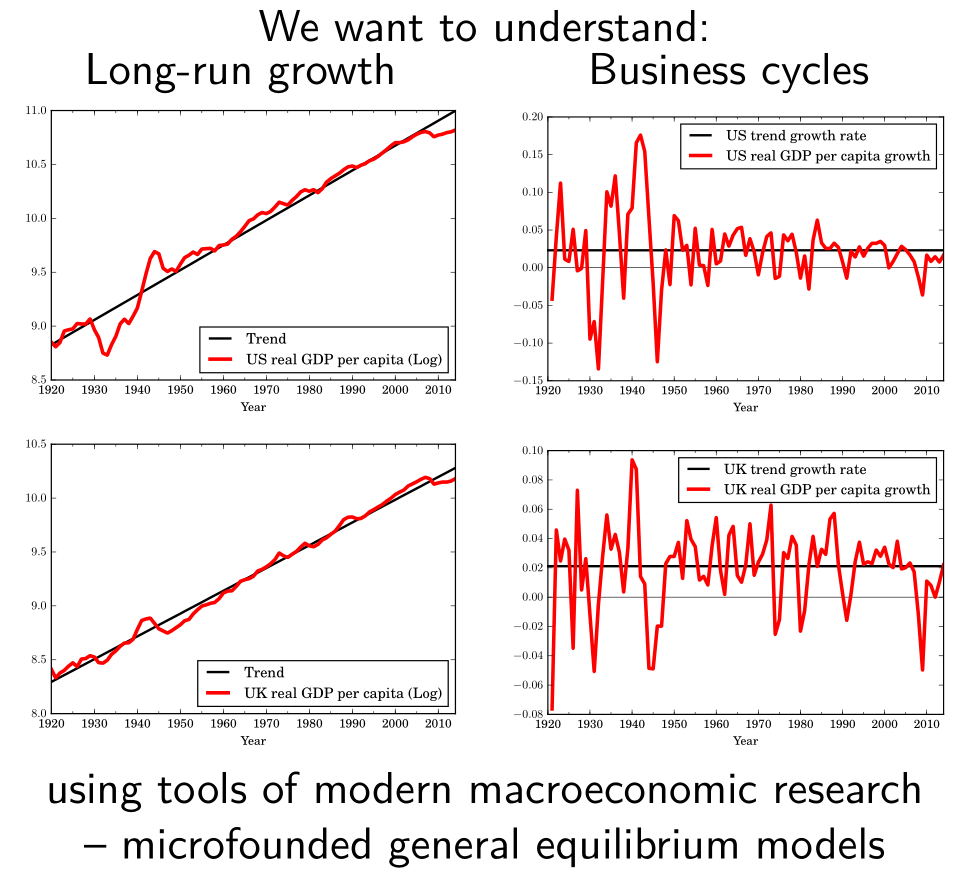
\includegraphics[scale = 0.4]{images/pol1}
\end{figure}
\end{frame}


\section{Decomposing time series: trend vs. cycle}

\begin{frame}
\frametitle{Trend vs Cycle: linear}
\begin{figure}
\centering
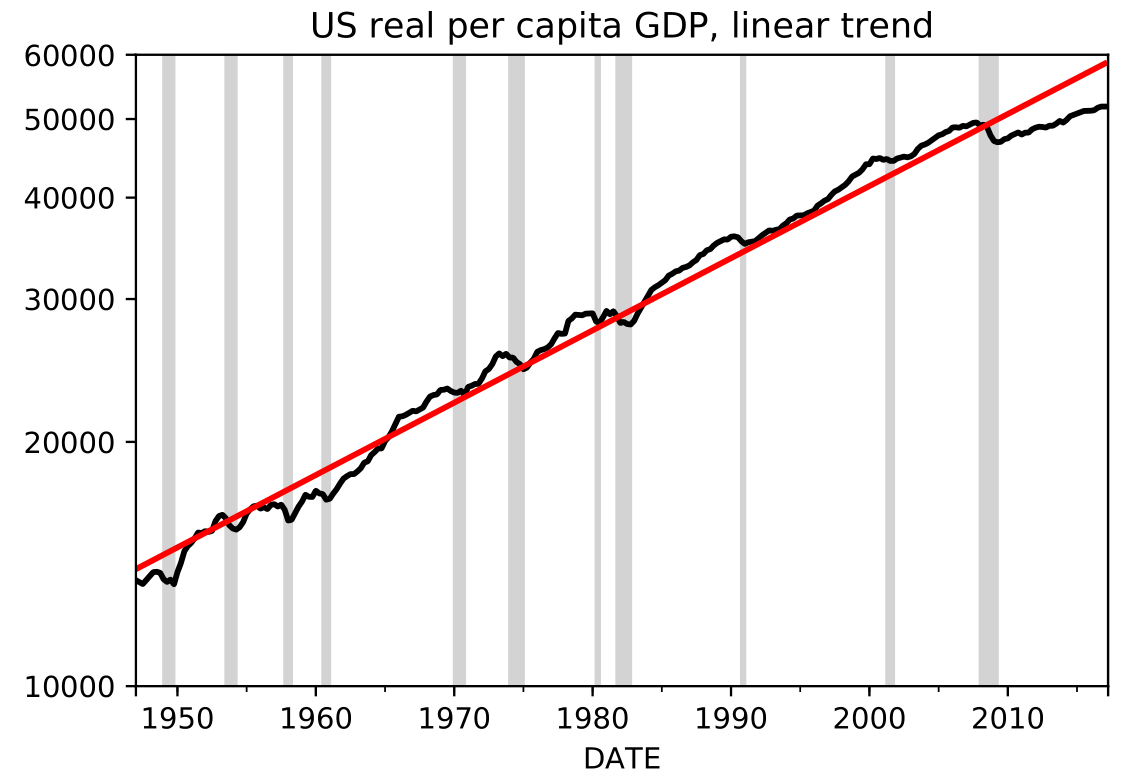
\includegraphics[scale = 0.4]{images/pol2}
\end{figure}
\end{frame}

\begin{frame}
\frametitle{Trend vs Cycle: linear}
\begin{figure}
\centering
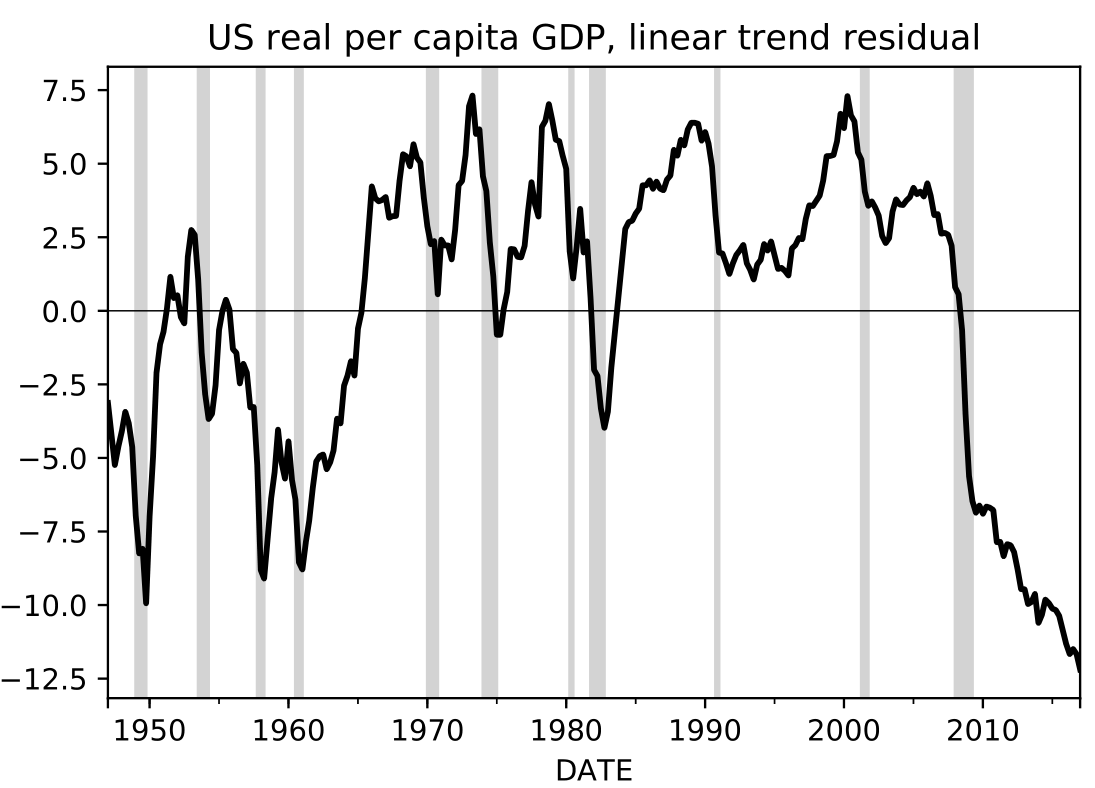
\includegraphics[scale = 0.4]{images/pol3}
\end{figure}
\end{frame}

\begin{frame}\frametitle{Trend vs Cycle: linear detrend}
\begin{figure}\centering
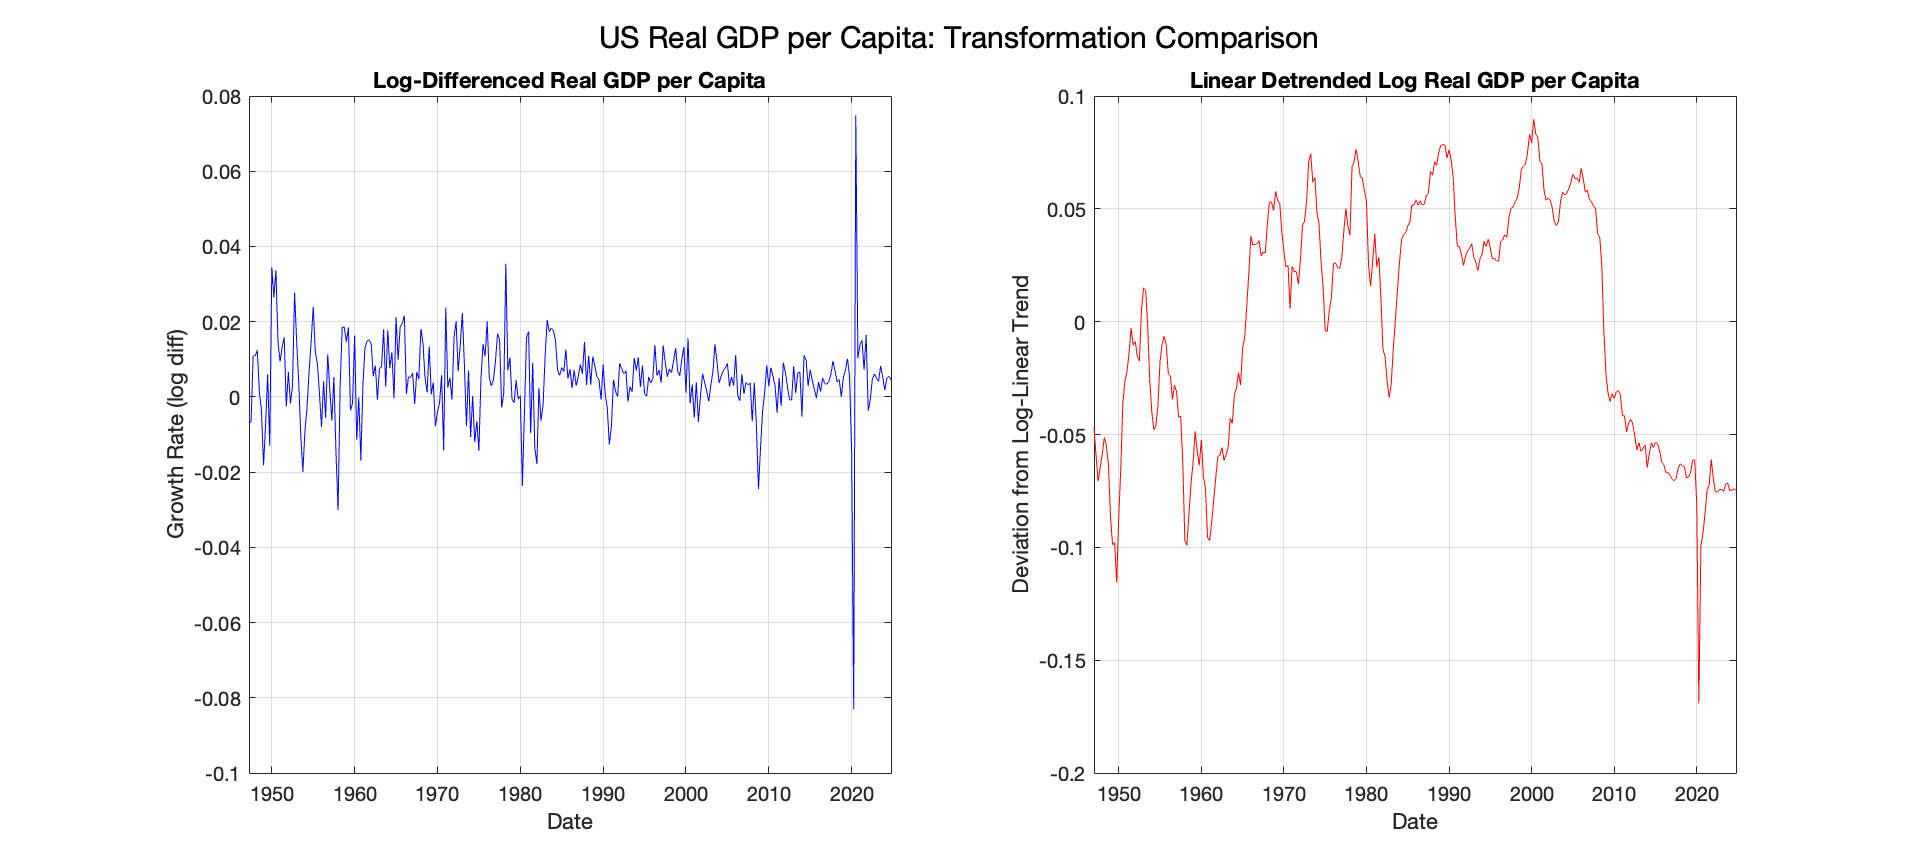
\includegraphics[width=\textwidth]{images/y_linear_detrend.png}
\end{figure}
\end{frame}


\begin{frame}
\frametitle{Trend vs Cycle: HP Filter}
\begin{figure}
\centering
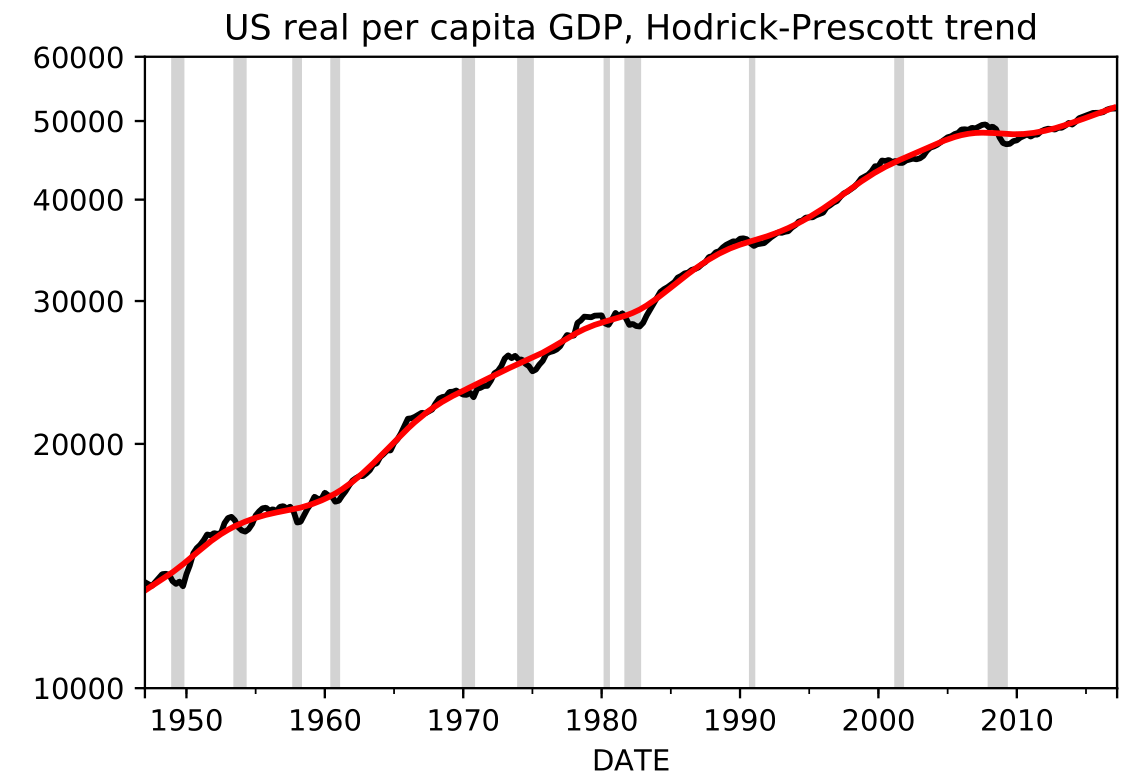
\includegraphics[scale = 0.4]{images/pol4}
\end{figure}
\end{frame}

\begin{frame}
\frametitle{Trend vs Cycle: HP Filter}
\begin{figure}
\centering
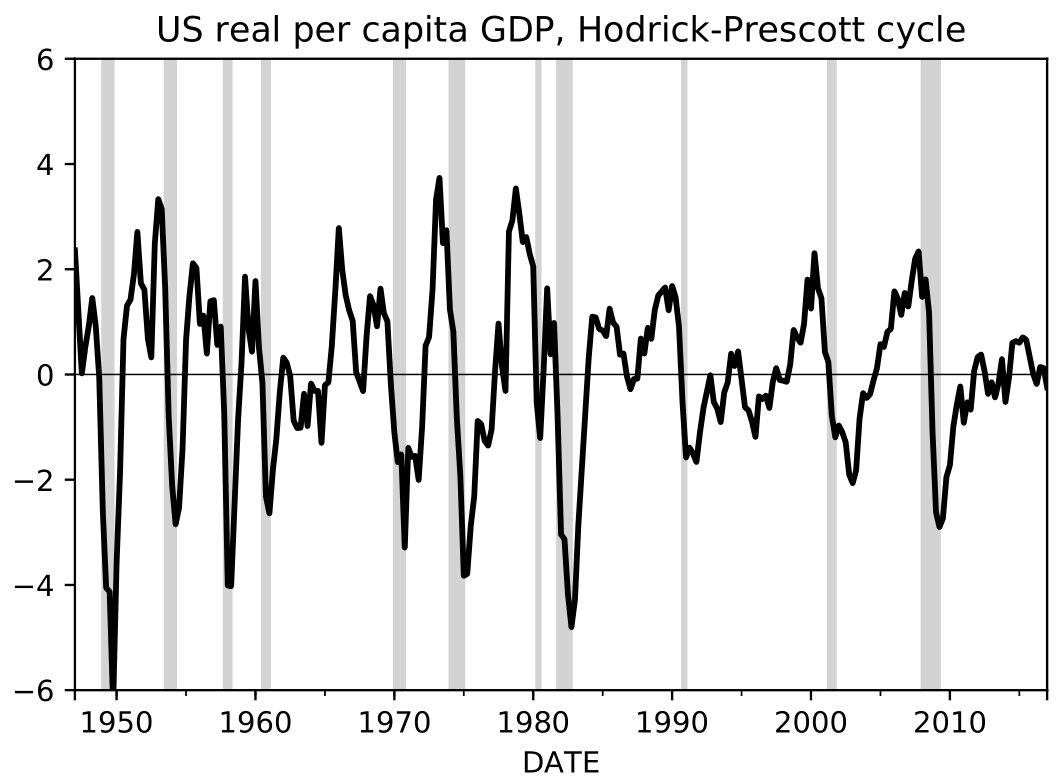
\includegraphics[scale = 0.4]{images/pol5}
\end{figure}
\end{frame}


\begin{frame}
\frametitle{Hodrick-Prescott Filter}
\begin{itemize}[<+->]
\item This next section is useful for your tutorial (tbc)
\item The Hodrick-Prescott filter is one of the most frequently used filters in macroeconomics
\item Considered to be a technique to obtain a \textbf{smoothed estimate} of the long term trend
\item Let $y_t$ denote the logarithm of a time series variable, for $t = 1,2 \ldots, T$
\item The series is then made up of trend component, $\tau_{t}$ and a cyclical component $c_{t}$, such that $y_{t} = \tau_{t} + c_{t}$, assuming some irregular (noise) component $\varepsilon_{t} \sim \mathcal{N}(0,\sigma)$
\item Given a chosen value of $\lambda$ there is a trend component that will solve the following minimisation problem
\end{itemize}
\end{frame}

\begin{frame}
\frametitle{Hodrick-Prescott Filter}
\small
\begin{itemize}[<+->]
\item The minimisation problem is,
\begin{align*}
\min_{t}\left(\sum_{t=1}^{T}(\underset{c_t}{\underbrace{y_{t} - \tau_{t}}})^{2} + \lambda\sum_{t=2}^{T-1}\left[(\tau_{t+1} - \tau_{t}) - (\tau_{t} - \tau_{t-1})\right]^{2}\right)
\end{align*}
\item First term is the sum of the squared deviations from the trend, \textbf{penalises movements away from the trend} (\textcolor{blue}{cyclical component})
\item Second term is a multiple, $\lambda$, of the sum of the \textbf{squares of the trend components second differences}
\item This term penalises variations in the growth rate of the trend component
\item Higher value of $\lambda \rightarrow$ higher penalty
\item All you really have to know here is that $\lambda$ controls the smoothness of the series estimate (i.e., $\lambda$ penalises the trend for `non-smoothness')
\item If $\lambda \rightarrow \infty$: \textbf{straight line}
\item If $\lambda \rightarrow 0$: \textbf{trend will lie on the series itself} because $y_{t} = \tau_{t}$ solves the minimisation problem
\end{itemize}
\end{frame}

\begin{frame}
\frametitle{HP Filter (two-sided)}
\begin{figure}
\centering
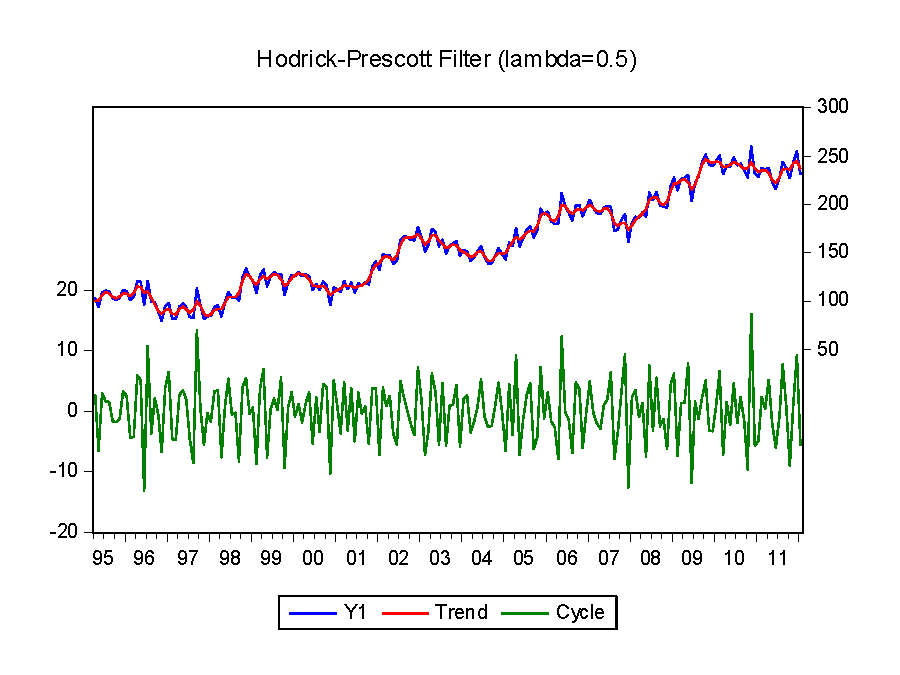
\includegraphics[width=9cm, height=9cm, keepaspectratio]{images/hp5}
\end{figure}
\end{frame}

\begin{frame}
\frametitle{HP Filter (two-sided)}
\begin{figure}
\centering
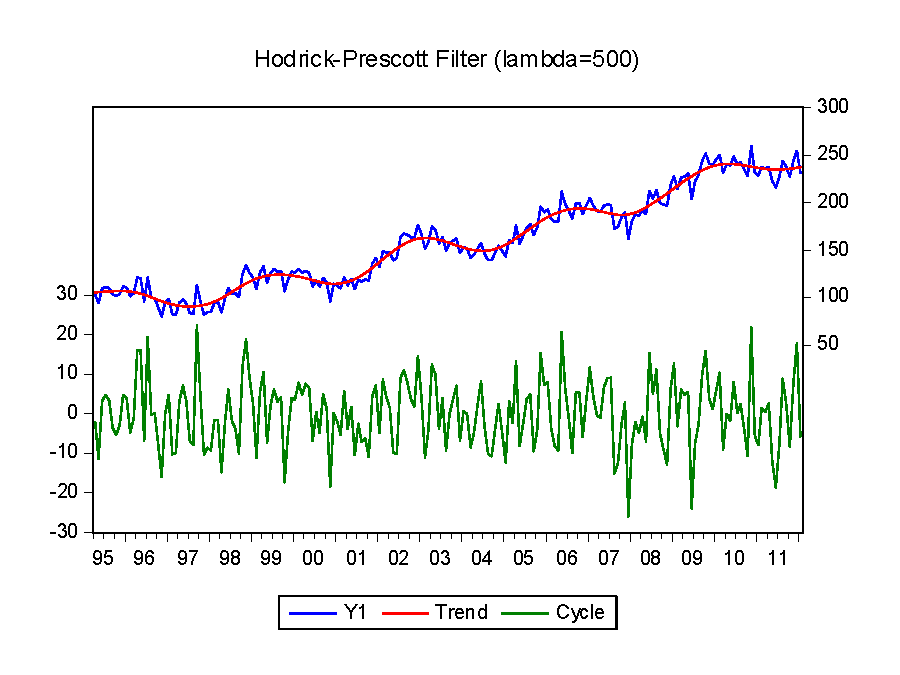
\includegraphics[width=9cm, height=9cm, keepaspectratio]{images/hp500}
\end{figure}
\end{frame}


\begin{frame}
\frametitle{HP Filter (two-sided)}
\begin{figure}
\centering
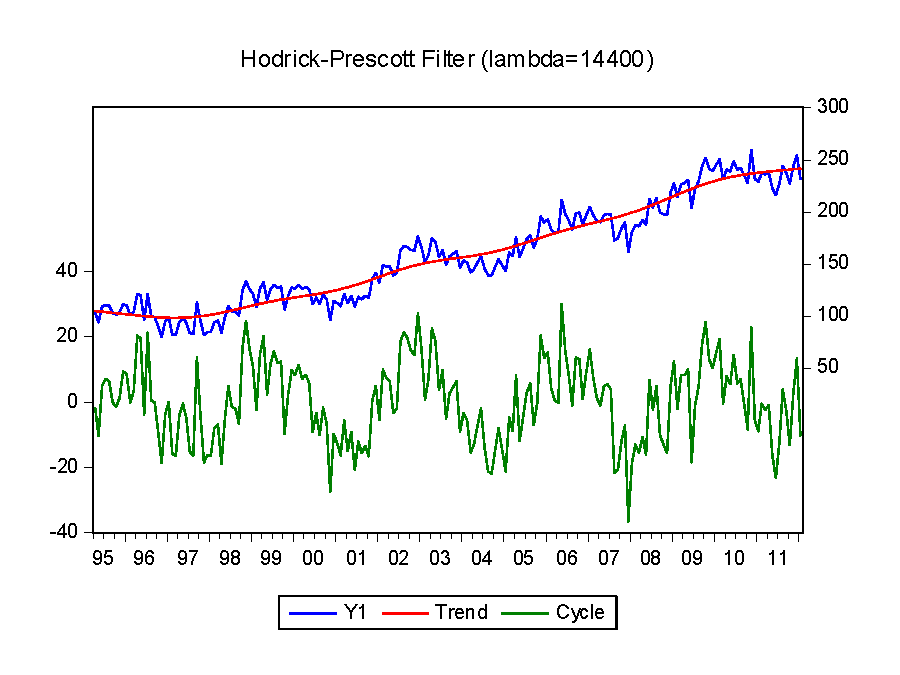
\includegraphics[width=9cm, height=9cm, keepaspectratio]{images/hp14400}
\end{figure}
\end{frame}



\begin{frame}
\frametitle{HP Filter (two-sided)}
\begin{figure}
\centering
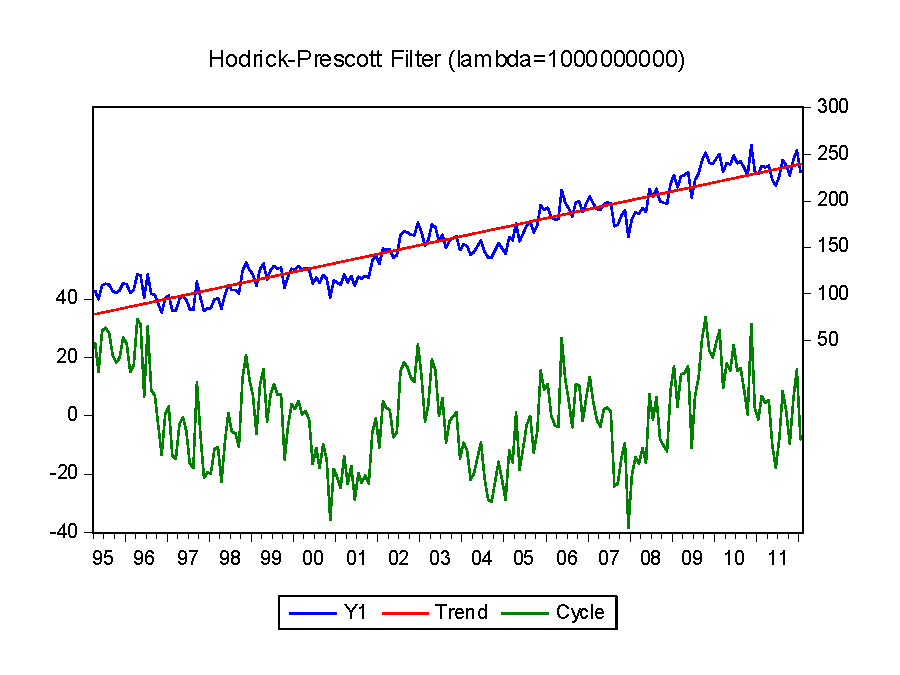
\includegraphics[width=9cm, height=9cm, keepaspectratio]{images/hp10}
\end{figure}
\end{frame}




\begin{frame}
\frametitle{Drawbacks to the HP filter}

\begin{itemize}
\item \textbf{Remark 12} (Non-Causal Filters): Thou shalt not use a non-causal, i.e. two-sided or Baxter-King, filter 
\item See Section 4.1 in Pfeifer (2024): \href{https://sites.google.com/site/pfeiferecon/dynare}{A Guide to Specifying Observation Equations for the Estimation of DSGE Models}
\item \href{https://en.wikipedia.org/wiki/Hodrick\%E2\%80\%93Prescott_filter}{Hamilton vs. Hodrick}
\item \href{https://uk.mathworks.com/videos/when-to-use-the-hodrick-prescott-filter-1678086873346.html?browser=F1help}{When to Use the Hodrick-Prescott Filter}
\end{itemize}

\end{frame}


\begin{frame}\frametitle{One-side vs. Two-sided HP filter}
\begin{figure}\centering
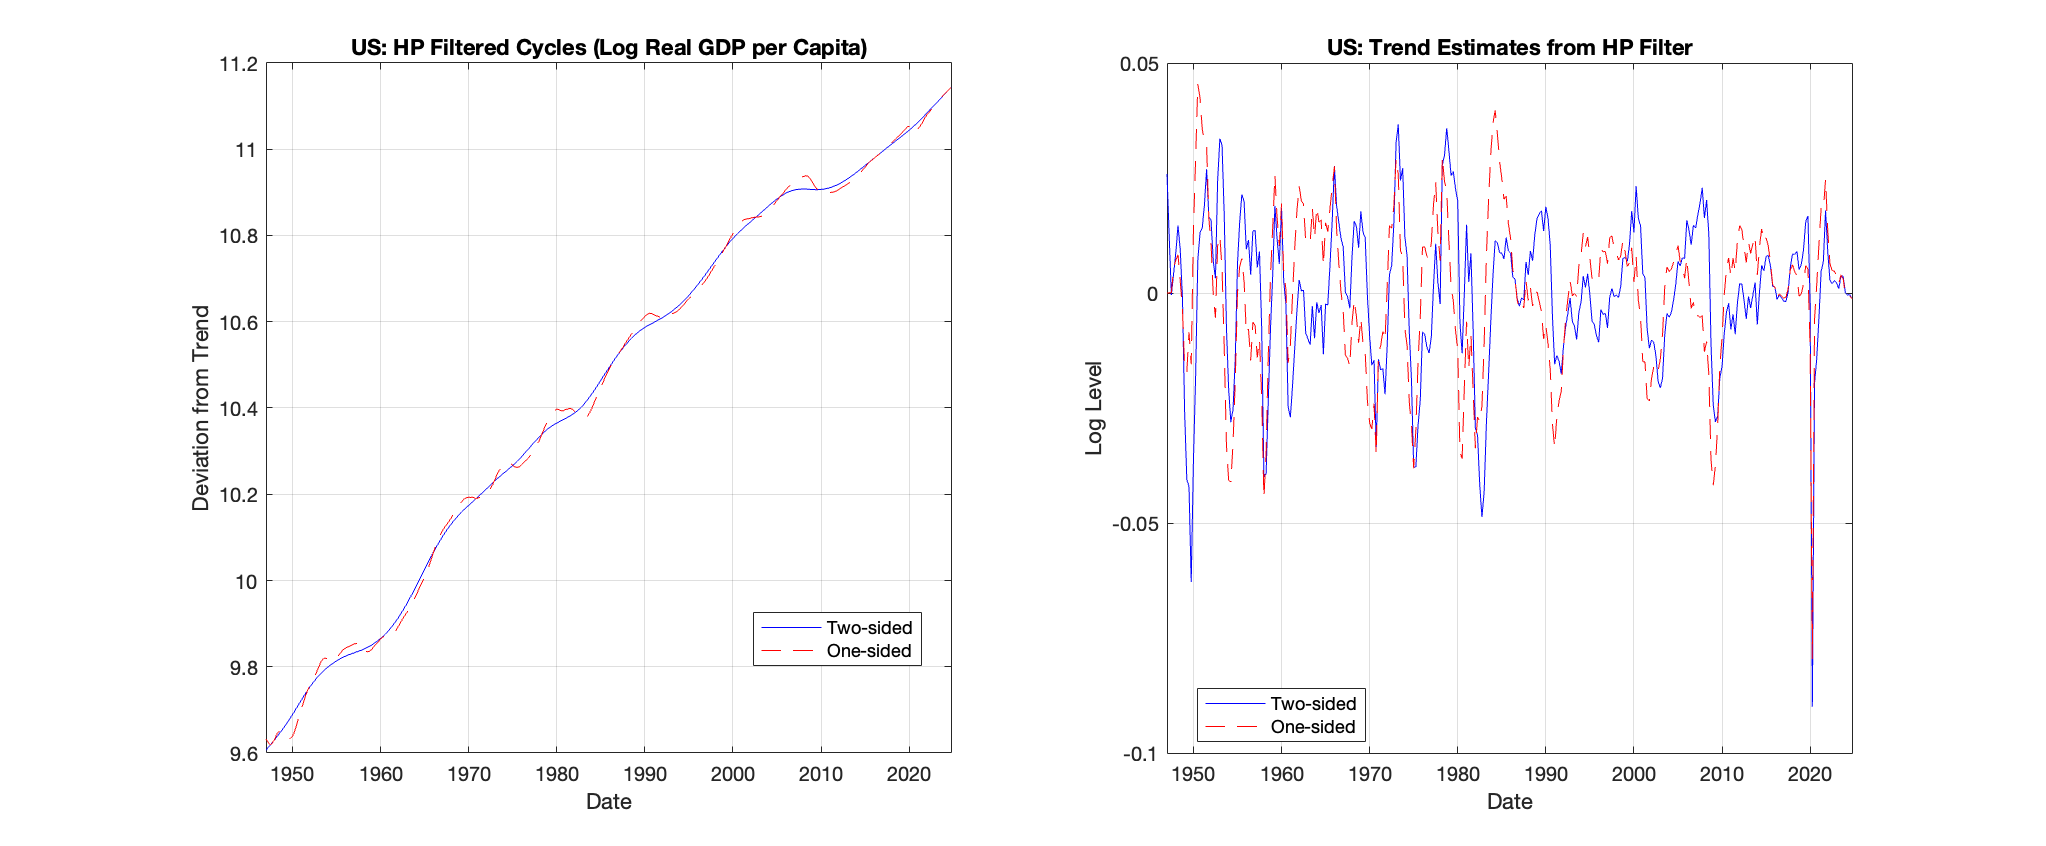
\includegraphics[width=1.1\textwidth]{images/y_hpfilter.png}
\end{figure}
\end{frame}

\begin{frame}\frametitle{One-side vs. Two-sided HP filter}
\begin{figure}\centering
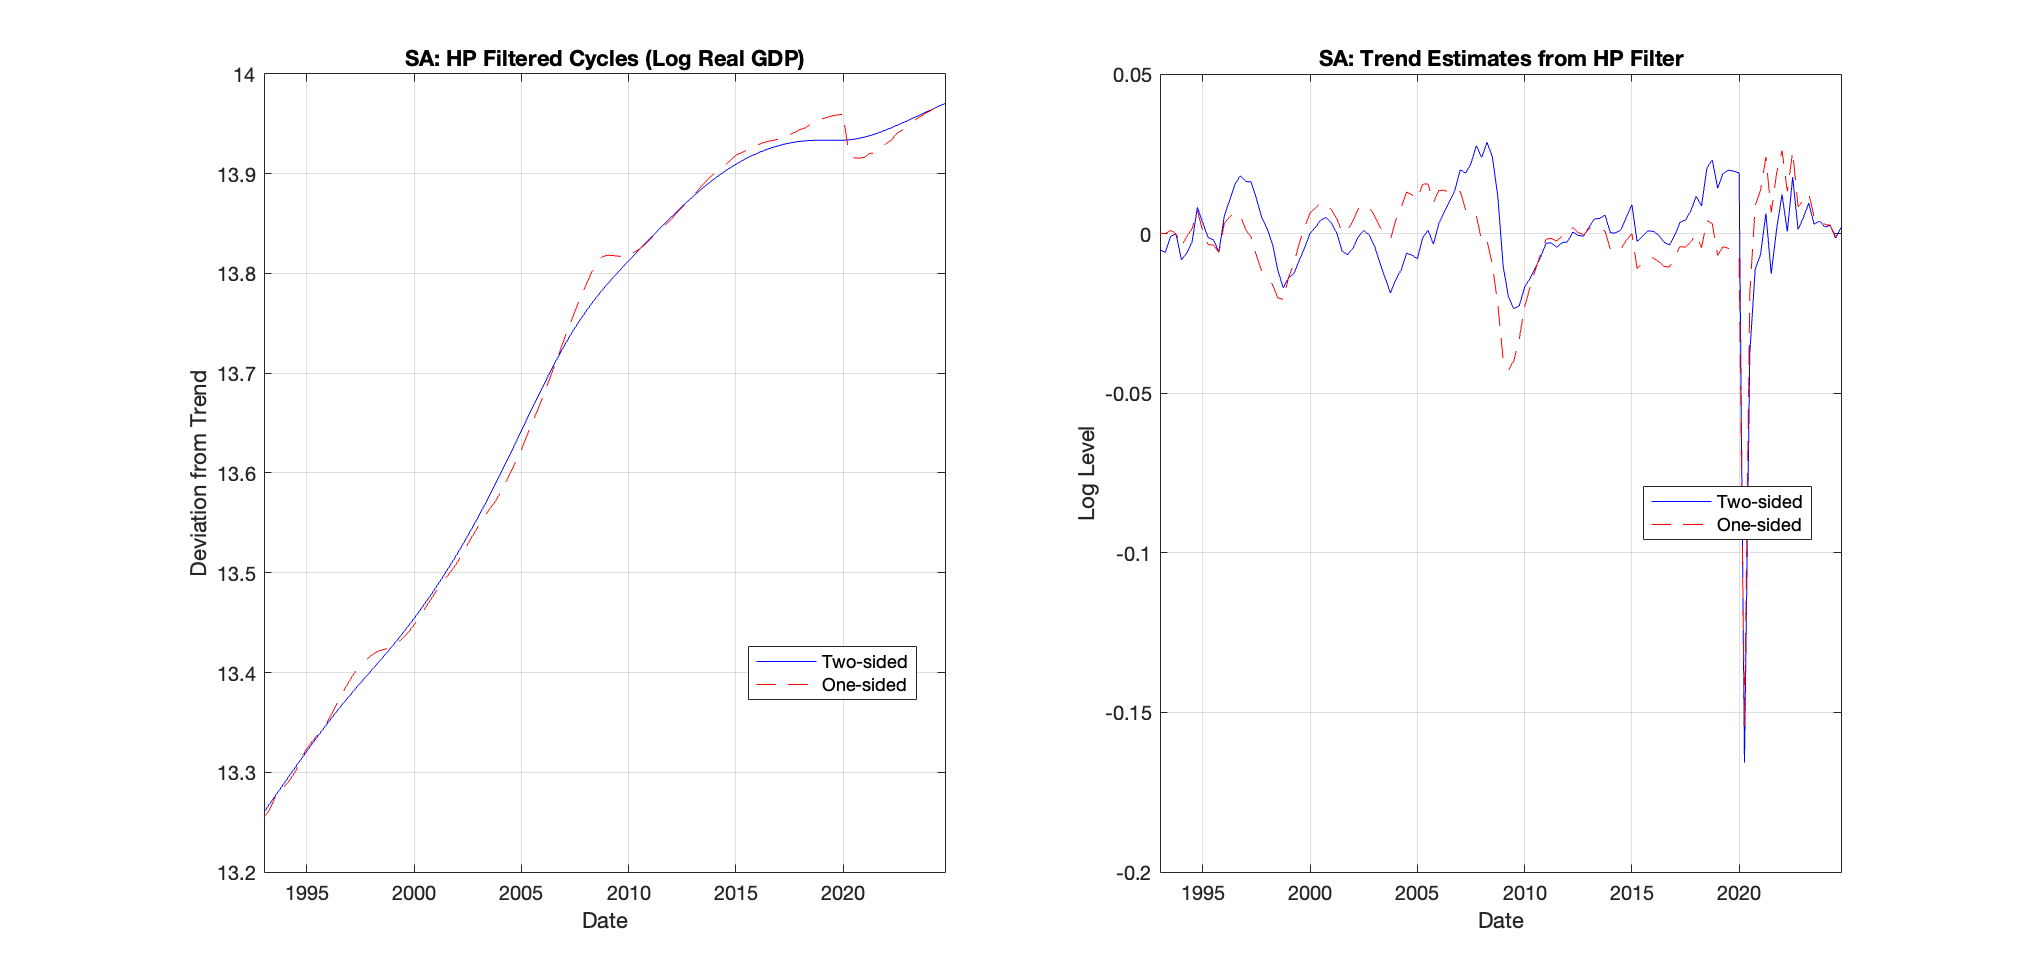
\includegraphics[width=1.1\textwidth]{images/y_sa_hpfilter.png}
\end{figure}
\end{frame}


\section{Goal of RBC models}


\begin{frame}
\frametitle{Goal of RBC models}
\begin{itemize}[<+->]
\item The goal of RBC models is to understand the sources and nature of aggregate fluctuations
\item Before the theories are presented, we will identify some of the major facts about short-run fluctuations.
\vspace{2mm}
\end{itemize}
\begin{enumerate}
\item Fluctuations do not exhibit any simple regular or cyclical pattern
\begin{itemize}
  \item Movements \textbf{not regular} $\rightarrow$ economy is perturbed by disturbances of various types and sizes at random intervals which propagate through the economy
  \item Major schools of economic thought differ on \textcolor{blue}{sources of shocks and propagation mechanisms}
\end{itemize}
\item Fluctuations are distributed unevenly over components of output
\item Asymmetries in output movement
\item Magnitude of fluctuations change over time.
\end{enumerate}
\end{frame}



\begin{frame}
\frametitle{Business cycle facts: USA 1948-2016}
\begin{figure}
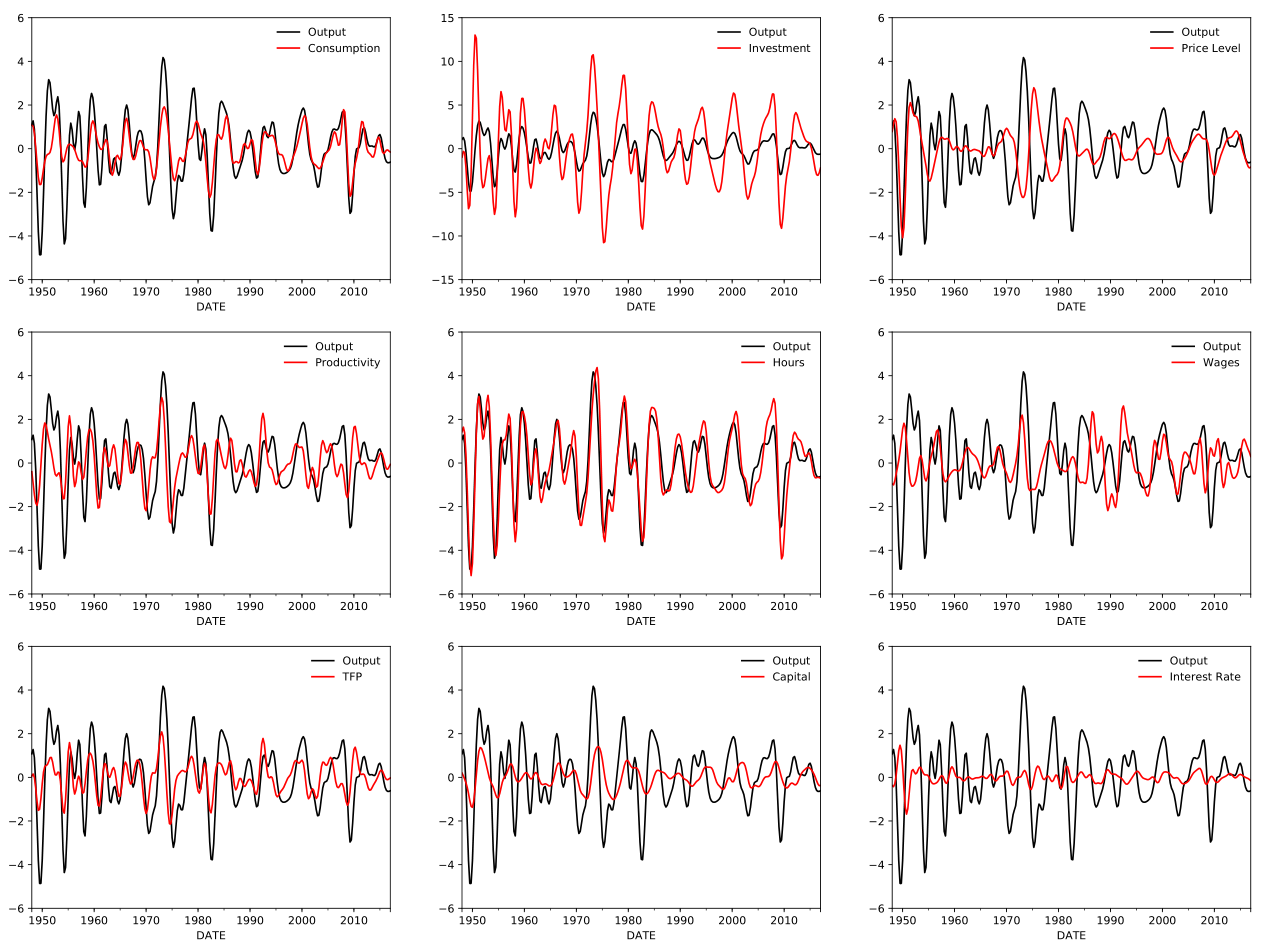
\includegraphics[scale = 0.4]{images/pol6}
\end{figure}
\end{frame}


\begin{frame}
\frametitle{Business cycle facts: USA 1948-2016}
\small
Here are some observations about the business cycle in the US.
\begin{itemize}[<+->]
\item Consumption is coincident, procyclical and less volatile than output
\item Investment is coincident, procyclical and more volatile than output
\item Price level can be procyclical and countercyclical
\item Productivity and TFP are both procyclical and leading output
\item Hours are slightly more volatile than output with 1-2 quarters lag
\item Real wage is procyclical when price level is countercyclical and countercyclical when price level is procyclical
\item Capital stock is procyclical, mildly volatile and lags output
\item Real interest rates are acyclical and the least volatile
\end{itemize}
\vspace{3mm}
Ideally, we would like our model to replicate these movements.
\end{frame}


\begin{frame}
\frametitle{Business cycle facts: USA 1948-2016}
\begin{figure}
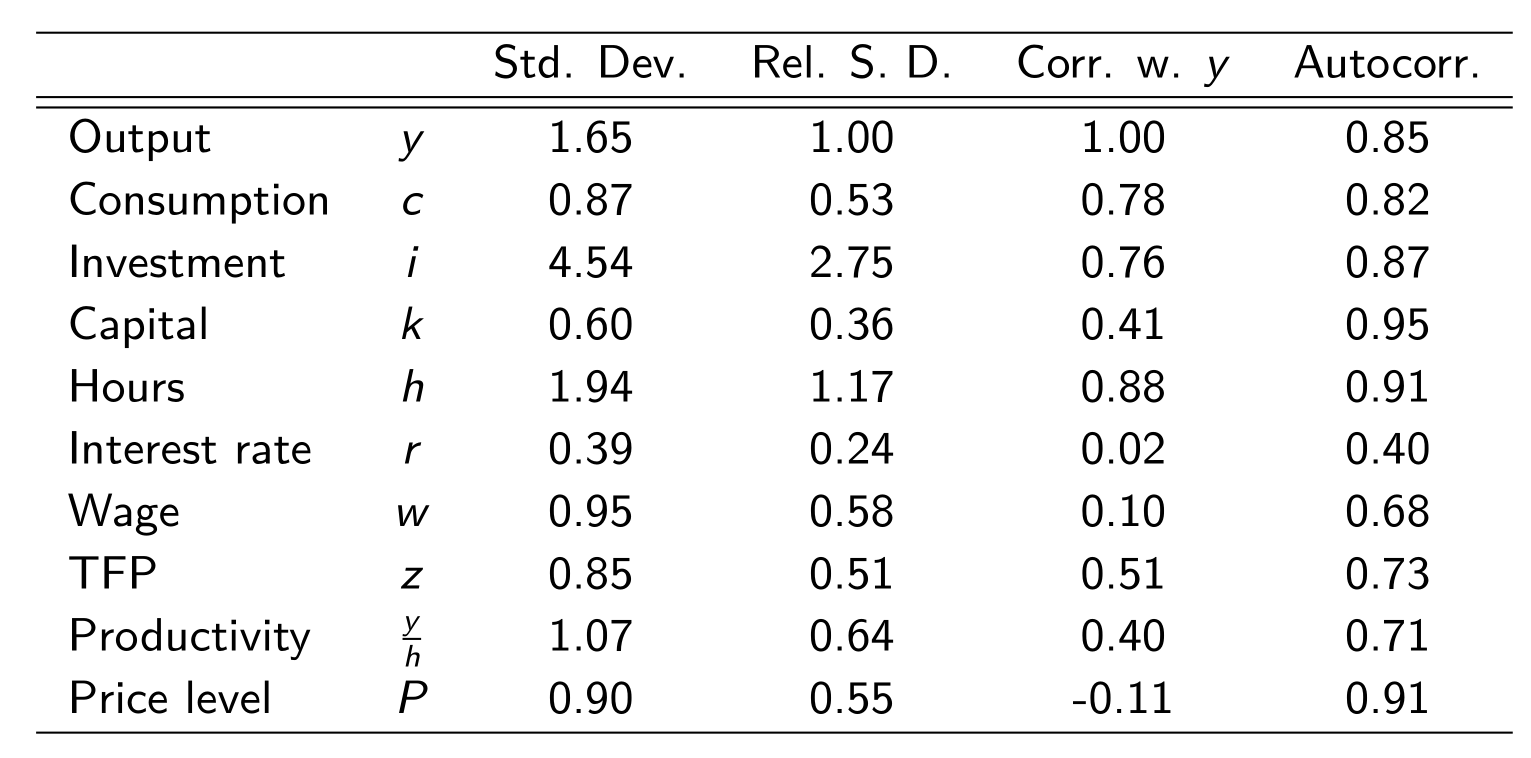
\includegraphics[scale = 0.33]{images/pol7}
\end{figure}
\end{frame}




\begin{frame}
\frametitle{Early RBC research}
\begin{itemize}[<+->]
\item Early research extended Ramsey model to incorporate aggregate fluctuations, which requires two modifications.
\begin{enumerate}
\item Introduce source of disturbances $\rightarrow$ without shocks model goes to BGP and grows smoothly
\item Allow for variations in employment (i.e. introduce a labour market)
\end{enumerate}
\vspace{2mm}
\item Two extensions suggested for the source of disturbances: (i) shocks to technology and (ii) changes in government purchases
\item Both of these shocks represent \textbf{real} disturbances!
\vspace{2mm}
\item In order to allow for employment variations we can include \textcolor{blue}{hours worked} in the households' utility function
\begin{itemize}
  \item Employment given by the intersection of labour demand and supply
\end{itemize}
\end{itemize}
\end{frame}


\section{Baseline RBC model}


\begin{frame}
\frametitle{Baseline RBC model (production)}
\begin{itemize}[<+->]
\item We will use a discrete-time variation of the Ramsey model.
\item Production function is Cobb-Douglas,
\begin{align*}
Y_{t} = K_{t}^{\alpha}(A_{t}L_{t})^{1-\alpha}, \quad 0 \leq \alpha \leq 1
\end{align*}
\item Capital stock in period $t+1$ is given by,
\begin{align*}
K_{t+1} &= K_{t} + I_{t} - {\delta}K_{t} \\
&= K_{t} + Y_{t} - C_{t} - G_{t} - \delta{K_{t}}, \quad \text{where} \quad Y_{t} = C_{t} + I_{t} + G_{t}
\end{align*}
\item Labour and capital are paid their marginal products,
\begin{align*}
w_{t} &= (1 - \alpha)\left(\frac{K_{t}}{A_{t}L_{t}}\right)^{\alpha}A_{t} \\
r_{t} &= \alpha\left(\frac{A_{t}L_{t}}{K_{t}}\right)^{1 - \alpha} - \delta
\end{align*}
\end{itemize}
\end{frame}


\begin{frame}
\frametitle{Baseline RBC model (consumption)}
\begin{itemize}[<+->]
\item Representative household maximises expected value of
\begin{align*}
U = {\sum_{t=0}^\infty}{e^{-\rho{t}}u(c_t, 1- l_{t})}{\frac{N_t}{H}}{d_t}
\end{align*}
where $u(\bullet)$ is the instantaneous utility function, $\rho$ is the discount rate, $N_{t}$ is population and $H$ is the number of households.
\item Population grows exogenously at rate $n$: $\ln{N_{t}} = \bar{N} + nt$.
\vspace{2mm}
\item Two arguments in the utility function $u(\bullet)$
\begin{itemize}
  \item Consumption per member of household, $c_{t}$
  \item Leisure per member $(1 - l_{t}) \rightarrow$ difference between time endowment ($1$) and amount each member works ($l_{t}$).
\end{itemize}
\vspace{2mm}
\item Specific functional form is \textbf{log-linear}: $u_{t} = \ln{c_{t}} + b\ln({1-l_{t}})$.
\end{itemize}
\end{frame}


\begin{frame}
\frametitle{Baseline RBC model (driving variables)}
\begin{itemize}[<+->]
\item Final assumption of the model concerns the behaviour of the driving variables: (i) technology and (ii) government purchases.
\vspace{3mm}
\item In the \textbf{absence of shocks}, trend growth in technology, $\ln{A_{t}}$, would be $\bar{A} + g_{t}$. Likewise, trend growth in per capita government purchases, $\ln{G_{t}}$, would be $\bar{G} + (n+g)t$.
\vspace{2mm}
\item We can, however, assume that technology (and/or government purchases) are subject to \textcolor{blue}{random disturbances}:
\begin{align*}
\ln{A_{t}} = \bar{A} + g_{t} + \tilde{A}_{t}
\end{align*}
where $\tilde{A}$ reflects departures from the trend and is assumed to follow an \textbf{AR(1)} process. In other words,
\begin{align*}
\tilde{A}_{t} = \rho_{A}\tilde{A}_{t-1} + \varepsilon_{A,t}, \quad -1 \leq \rho_{A} \leq 1
\end{align*}
where $\varepsilon_{A,t}$ are white noise disturbances. The equation shows that the effect of shocks disappear gradually over time.
\end{itemize}
\end{frame}


\subsection{Household behaviour: three cases}

\begin{frame}
\frametitle{Household behaviour}
\begin{itemize}[<+->]
\item For this section we will evaluate household behaviour at differing levels of complexity.
\vspace{3mm}
\item We will consider three different cases.
\begin{enumerate}
\item \textbf{Case 1}: Household lives for one period
\item \textbf{Case 2}: Household lives for two periods
\item \textbf{Case 3}: Household lives for two periods and there is uncertainty
\end{enumerate}
\vspace{3mm}
\item We will then extend this to a more general case, which is quite tricky.
\end{itemize}
\end{frame}


\begin{frame}
\frametitle{Household behaviour: Case 1}
\small
\begin{itemize}[<+->]
\item The budget constraint for this case is simple. Since the household (one member) does not save (i.e., no wealth), we have $c_{t} \leq w_{t}l_{t}$.
\item This means that the optimisation problem is,
\begin{align*}
\mathcal{L} = \ln{c_{t}} + b\ln(1-l_{t}) + \lambda_{t}(w_{t}l_{t} - c_{t}) ,
\end{align*}
where the household chooses $c_{t}$ and $l_{t}$ to maximize utility.
\item First order conditions for this problem are then,
\begin{align*}
&\mathcal{L}_{c} : \frac{1}{c_{t}} - \lambda_{t} = 0 \\
&\mathcal{L}_{l} : -b\left(\frac{1}{1 - l_{t}}\right) + \lambda_{t}w_{t} = 0 \\
&\mathcal{L}_{\lambda} : w_{t}l_{t} - c_{t} = 0
\end{align*}
\item Combining the first two equations, we have the following:
\begin{align*}
\frac{1}{l_{t}} = b\left(\frac{1}{1 - l_{t}}\right)
\end{align*}
\item Labour-leisure choice is independent of wage; only depends on the weight of leisure, $b$, in utility.
\end{itemize}
\end{frame}

\begin{frame}
\frametitle{Household behaviour: Case 2}
\small
\begin{itemize}[<+->]
\item Household lives for two periods
\item Continue to assume that it has no initial wealth and that it has only one member
\item In addition, assume that there is no uncertainty about the interest rate or the
second-period wage.
\item Budget constraint for this problem is now,
\begin{align*}
c_{t} + \frac{1}{1+r_{t+1}}c_{t+1} = w_{t}l_{t} + \frac{w_{t+1}l_{t+1}}{1+r_{t+1}}
\end{align*}
\item The Lagrangian for this problem is (note: $\beta = e^{-\rho}$),
\begin{align*}
\mathcal{L} = &\ln{c_{t}} + b\ln(1-l_{t}) + \beta[\ln{c_{t+1}} + b\ln({1 - l_{t+1}})] + \\
& \lambda_{t}\left(w_{t}l_{t} + \frac{w_{t+1}l_{t+1}}{1+r_{t+1}} - c_{t} - \frac{1}{1+r_{t+1}}c_{t+1} \right)
\end{align*}
where the four choice variables are $c_{t}, c_{t+1}, l_{t}$ and $l_{t+1}$.
\end{itemize}
\end{frame}

\begin{frame}
\frametitle{Household behaviour: Case 2}
\small
\begin{itemize}[<+->]
\item First order conditions for this problem are:
\begin{align*}
&\mathcal{L}_{c_t} : \frac{1}{c_{t}} - \lambda_{t} = 0 \\
&\mathcal{L}_{c_{t+1}} : \beta\frac{1}{c_{t+1}} - \lambda_{t}\left(\frac{1}{1 + r_{t+1}}\right) = 0\\
&\mathcal{L}_{l_t} : -b\left(\frac{1}{1 - l_{t}}\right) + \lambda_{t}w_{t} = 0 \\
&\mathcal{L}_{l_{t+1}} : -b\beta\left(\frac{1}{1 - l_{t+1}}\right) + \lambda_{t}\frac{w_{t}}{1+r_{t+1}} = 0
\end{align*}
\item Combining the first two FOCs we get the  \textbf{Euler equation},
\begin{align*}
\frac{1}{c_{t}} = \beta{(1+r_{t+1})}\frac{1}{c_{t+1}}
\end{align*}
\item The third and fourth FOCs can be combined to form,
\begin{align*}
\frac{(1-l_t)}{(1-l_{t+1})} = \frac{1}{\beta{(1+r_{t+1})}}\frac{w_{t+1}}{w_{t}}
\end{align*}
\item This equation shows that households will substitute labour across time.
\item Response of labour supply to relative wages and interest rates is known as the \textbf{intertemporal substitution} in labour supply.
\end{itemize}
\end{frame}

\begin{frame}
\frametitle{Household behaviour: Case 3}
\small
\begin{itemize}[<+->]
\item For the third case there are two general approaches. Romer uses one method, I will stick to Lagrangians.
\begin{align*}
\mathcal{L} = &\ln{c_{t}} + b\ln(1-l_{t}) + \beta\mathbb{E}_{t}[\ln{c_{t+1}} + b\ln({1 - l_{t+1}})] + \\
& \lambda_{t}\left(w_{t}l_{t} + \mathbb{E}_{t}\left[\frac{w_{t+1}l_{t+1}}{1+r_{t+1}}\right] - c_{t} - \mathbb{E}_{t}\left[\frac{1}{1+r}c_{t+1}\right] \right)
\end{align*}
\item From the first order conditions, the Euler equation will be,
\begin{align*}
\frac{1}{c_{t}} = \beta\mathbb{E}_{t}\left[{(1+r_{t+1})}\frac{1}{c_{t+1}}\right]
\end{align*}
\item Cannot seperate the two terms on the right-hand side because $c_{t+1}$ and $r_{t+1}$ might be correlated.
\item Combining FOCs for labour supply and consumption we get,
\begin{align*}
\frac{c_{t}}{(1-l_{t})} = \frac{w_{t}}{b}
\end{align*}
\item Interesting to note that uncertainty does not enter into the labour choice.
\end{itemize}
\end{frame}

\subsection{An analytical special case}

\begin{frame}
\frametitle{Special case of the model}
\begin{itemize}[<+->]
\item The model we constructed cannot be solved analytically. So we will look at a \textbf{simplified version} of the model.
\item Two changes: (i) eliminate government and (ii) $100\%$ depreciation
\item Evolution of capital stock and real interest rate become,
\begin{align*}
K_{t+1} &= Y_{t} - C_{t} \\
1 + r_{t} &= \alpha\left(\frac{A_{t}L_{t}}{K_{t}}\right)^{1 - \alpha}
\end{align*}
\vspace{2mm}
\item To solve this type of model I will show you a method in class.
\end{itemize}
\end{frame}


\begin{frame}
\frametitle{Special case of the model}
\small
\begin{itemize}[<+->]
\item From the new method we determined that the following holds,
\begin{align*}
\frac{1}{c_{t}} = e^{-\rho}\mathbb{E}_{t}\left[\frac{1+r_{t+1}}{c_{t+1}}\right]
\end{align*}
\item Since $c_{t} = (1 - s_{t})Y_{t}/N_{t}$, we can rewrite this as,
\begin{align*}
\frac{1}{(1 - s_{t})Y_{t}/N_{t}} &= e^{-\rho}\mathbb{E}_{t}\left[\frac{1+r_{t+1}}{(1 - s_{t+1})Y_{t+1}/N_{t+1}}\right] \\
-\ln{(1 - s_{t})Y_{t}/N_{t}} &= {-\rho} + \ln\mathbb{E}_{t}\left[\frac{1+r_{t+1}}{(1 - s_{t+1})Y_{t+1}/N_{t+1}}\right] \\
-\ln{(1 - s_{t})Y_{t}/N_{t}} &= {-\rho} + \ln\mathbb{E}_{t}\left[\frac{\alpha{Y_{t+1}}}{(1 - s_{t+1})K_{t+1}Y_{t+1}/N_{t+1}}\right] \\
-\ln{(1 - s_{t})Y_{t}/N_{t}} &= {-\rho} + \ln\mathbb{E}_{t}\left[\frac{{\alpha}N_{t+1}}{(1 - s_{t+1})s_{t}Y_{t}}\right] \\
\end{align*}
\item Finally this gives us,
\begin{align*}
&-\ln(1-s_{t}) - \ln{Y_{t}} + \ln{N_{t}} \\
&= -\rho + \ln\alpha + \ln{N_{t}} + n - \ln{s_{t}} - \ln{Y_{t}} + \ln{\mathbb{E}_{t}}\left[\frac{1}{1-s_{t+1}}\right]
\end{align*}
\end{itemize}
\end{frame}

\begin{frame}
\frametitle{Special case of the model}
\begin{align*}
\ln{s_{t}}-\ln(1-s_{t}) = -\rho + \ln\alpha + n + \ln{\mathbb{E}_{t}}\left[\frac{1}{1-s_{t+1}}\right]
\end{align*}
\begin{itemize}[<+->]
\item \textbf{Important}: The two state variables, $A$ and $K$ don't enter this equation (i.e. can get growth path without them)
\item If $s$ is constant at some value $\hat{s}$, then $s_{t+1}$ is not uncertain and $\ln{\mathbb{E}_{t}}\left[{1}/{1-s_{t+1}}\right]$ simply becomes ${1}/{(1-\hat{s})}$.
\vspace{4mm}
\item The result is that $\ln{\hat{s}} = \ln{\alpha} + n - \rho$ or $\hat{s} = \alpha{e^{n-\rho}}$.
\item Model has a solution where the savings rate is constant.
\end{itemize}
\end{frame}

\begin{frame}
\frametitle{Special case of the model}
\begin{itemize}[<+->]
\item From the new method we also determined that $c_{t}/(1-l_{t}) = w_{t}/b$.
\item Since $c_{t} = C_{t}/N_{t} = (1 - \hat{s})Y_{t}/N_{t}$, we can write
\begin{align*}
(1 - \hat{s})Y_{t}/N_{t}/(1-l_{t}) &= w_{t}/b \\
\ln(1 - \hat{s})Y_{t}/N_{t} - \ln(1-l_{t}) &= \ln{w_{t}} - \ln{b}
\end{align*}
\item Since the production function is Cobb-Douglas, we have that $w_{t} = (1-\alpha)Y_{t}/(l_{t}N_{t})$, which yields,
\begin{align*}
\ln{l}_{t} - \ln(1-l_{t})
= \ln{1-\alpha} + \ln{Y}_{t} - \ln(1 - \hat{s}) - \ln{b}
\end{align*}
\item Rewriting this, we get,
\begin{align*}
l_{t} = \frac{1-\alpha}{(1-\alpha) + b(1-\hat{s})}
\end{align*}
which indicates to us that $l_{t} = \hat{l}$ is also a constant.
\end{itemize}
\end{frame}


\begin{frame}
\frametitle{Special case of the model}
\begin{itemize}[<+->]
\item We need to assess output fluctuations from the dynamics of technology and behaviour of capital stock.
\item If we take the natural logarithm of the production function, $Y_{t} = K_{t}^{\alpha}(A_{t}L_{t})^{1-\alpha}$ we have,
\begin{align*}
\ln{Y_{t}} &= \alpha\ln{K_{t}} + (1-\alpha)(\ln{A_{t}} + \ln{L_{t}}) \\
 &= \alpha\ln{\hat{s}} + \alpha\ln{Y_{t-1}} + (1-\alpha)(\ln{A_{t}} + \ln{\hat{l}} +  \ln{N_{t}}) \\
 &= \alpha\ln{\hat{s}} + \alpha\ln{Y_{t-1}} + (1-\alpha)(\ln{A_{t}} + \ln{\hat{l}} +  \ln{N_{t}}) \\
 &= \alpha\ln{\hat{s}} + \alpha\ln{Y_{t-1}} + (1-\alpha)(\bar{A} + gt + \tilde{A} + \ln{\hat{l}} +  \bar{N} + nt)
\end{align*}
\item We can define a new variable $\tilde{Y}$ to be the deviation of the log of output ($\ln{Y_{t}}$) from its ``no shock'' value.
\item ``No shock'' value is the one that would occur if shocks were zero.
\end{itemize}
\end{frame}

\begin{frame}
\frametitle{Special case of the model}
\begin{itemize}[<+->]
\item Decompose $Y$ into a \textbf{trend and cyclical} component.
\item We define $\bar{Y}_{t}$ to be the no-shock (trend) level of the log of output.
\item This would mean that $\tilde{Y}_{t} \equiv \ln{Y_{t}} - \bar{Y}_{t}$ is the cyclical component.
\item If all shocks were zero, then $\tilde{A}_{t} = 0$ and $\ln{Y_{t-1}} = \bar{Y}_{t-1}$.
\vspace{3mm}
\item From this simplification (and the equation on the previous slide) we can get an equation for $\bar{Y}_{t}$.
\begin{align*}
\bar{Y}_{t} = \alpha\ln{\hat{s}} + \alpha\bar{Y}_{t-1} + (1-\alpha)(\bar{A} + gt) + (1-\alpha)(\ln{\hat{l}} +  \bar{N} + nt)
\end{align*}
\item By extension we have an equation for $\tilde{Y}_{t}$, given by:
\begin{align*}
\tilde{Y}_{t} = \ln{Y_{t}} - \bar{Y}_{t} &= \alpha(\ln{Y_{t-1}} - \bar{Y}_{t-1}) + (1-\alpha)\tilde{A}_{t}  \\
&= \alpha\tilde{Y}_{t-1} + (1-\alpha)\tilde{A}_{t}
\end{align*}
which is the equation in the textbook.
\end{itemize}
\end{frame}

\begin{frame}
\frametitle{Special case of the model}
\small
\begin{itemize}[<+->]
\item Since this equation holds each period it implies that
\begin{align*}
\tilde{Y}_{t}  &= \alpha\tilde{Y}_{t-1} + (1-\alpha)\tilde{A}_{t} \\
\tilde{Y}_{t-1} &= \alpha\tilde{Y}_{t-2} + (1-\alpha)\tilde{A}_{t-1}
\end{align*}
\item This can then be rewritten in terms of $\tilde{A}_{t-1}$ as:
\begin{align*}
\tilde{A}_{t-1} = \frac{1}{1-\alpha}\left(\tilde{Y}_{t-1} - \alpha\tilde{Y}_{t-2}\right)
\end{align*}
\item We also know from our definition at the beginning that $\tilde{A}_{t} = \rho_A\tilde{A}_{t-1} + \varepsilon_{A,t}$. Combining these equations we have:
\begin{align*}
\tilde{Y}_{t} &= \alpha\tilde{Y}_{t-1} + (1-\alpha)(\rho_A\tilde{A}_{t-1} + \varepsilon_{A,t}) \\
&= \alpha\tilde{Y}_{t-1} + (1-\alpha)\left[\frac{\rho_{A}}{1-\alpha}\left(\tilde{Y}_{t-1} - \alpha\tilde{Y}_{t-2}\right) + \varepsilon_{A,t}\right] \\
&= \alpha\tilde{Y}_{t-1} + \rho_{A}\left(\tilde{Y}_{t-1} - \alpha\tilde{Y}_{t-2}\right) + (1-\alpha)\varepsilon_{A,t} \\
&= (\alpha + \rho_{A})\tilde{Y}_{t-1} - \alpha\rho_{A}\tilde{Y}_{t-2} + (1-\alpha)\varepsilon_{A,t}
\end{align*}
\item We see here that $\tilde{Y}_{t}$ can be written as a linear combination of two lags and a white noise disturbance term.
\end{itemize}
\end{frame}



\begin{frame}
\frametitle{Special case of the model}
\begin{align*}
\tilde{Y}_{t} = (\alpha + \rho_{A})\tilde{Y}_{t-1} - \alpha\rho_{A}\tilde{Y}_{t-2} + (1-\alpha)\varepsilon_{A,t}
\end{align*}
The combination of positive coefficient in the first lag and negative coefficient in the second lag can cause output to have a \textbf{hump-shaped} response to disturbances.
\begin{figure}[h]
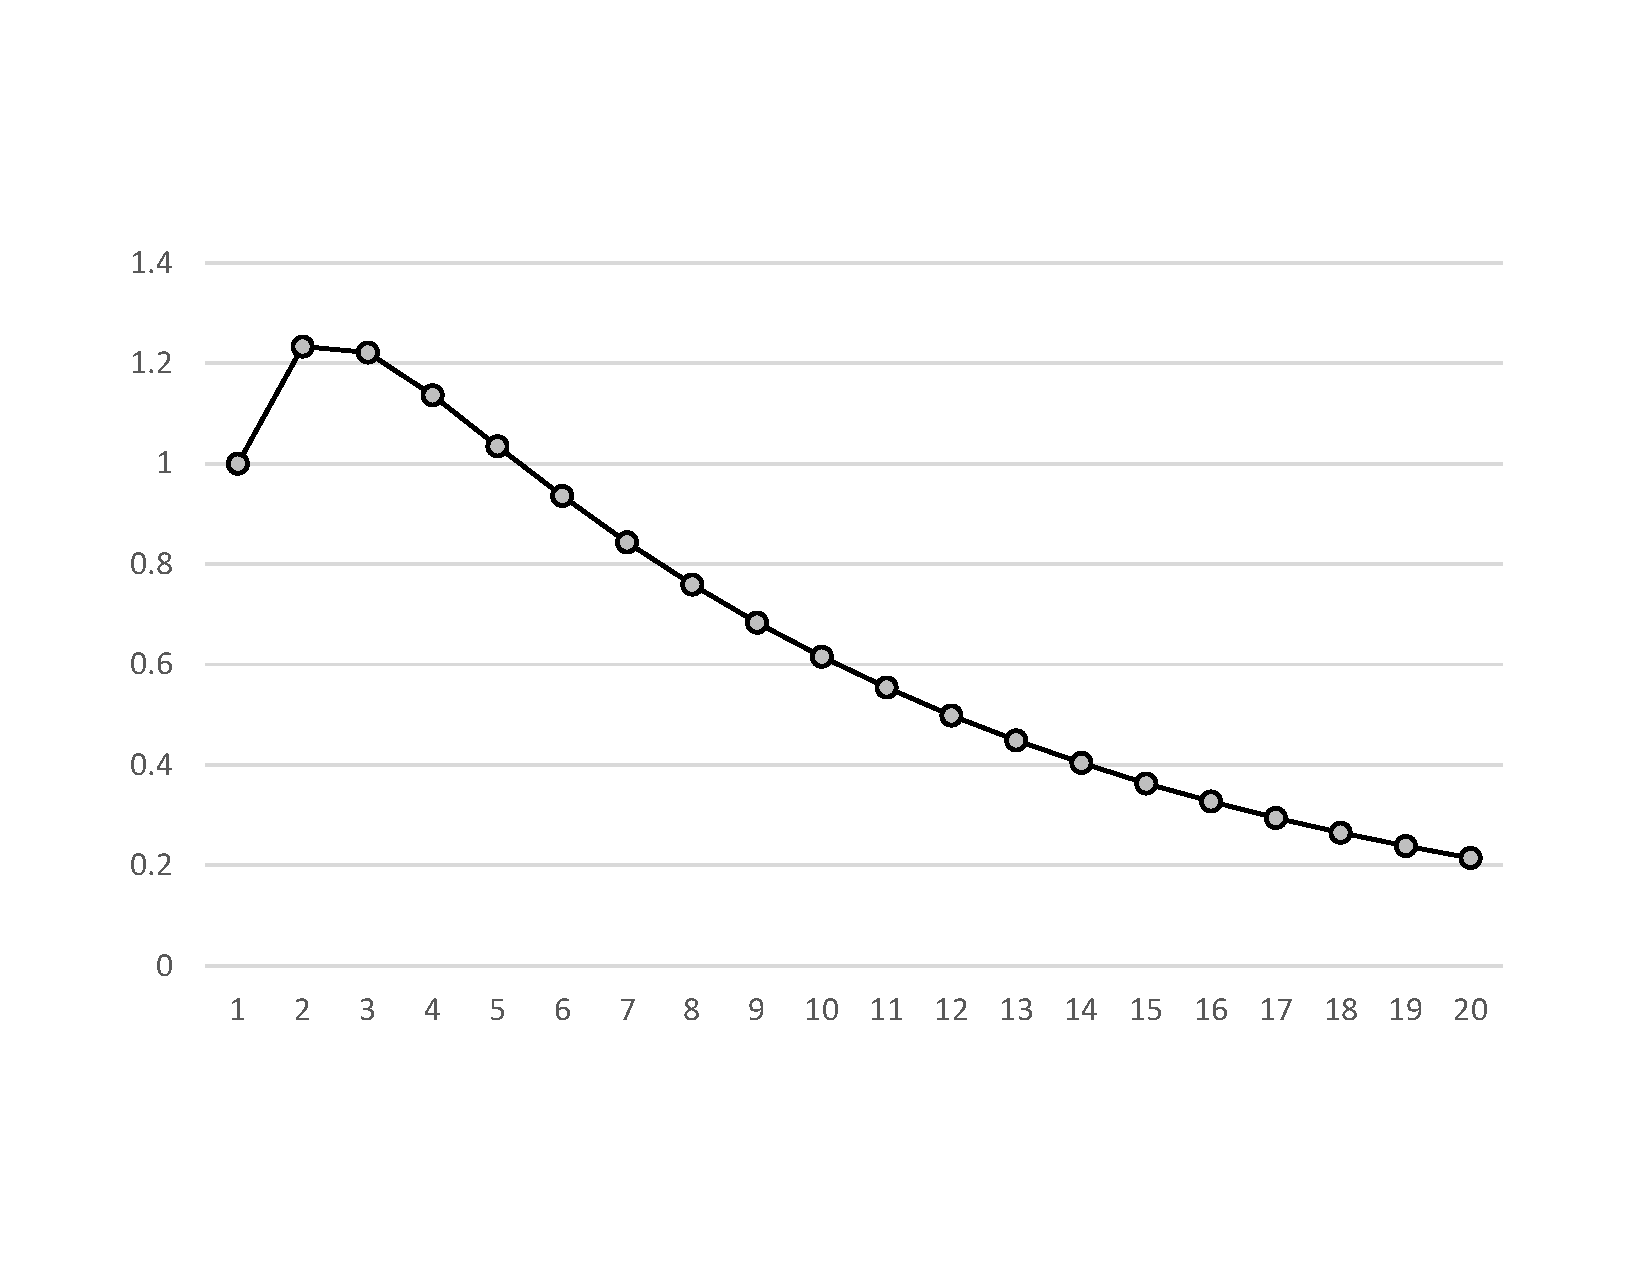
\includegraphics[scale = 0.3]{images/output-shock}
\end{figure}
\end{frame}

\begin{frame}
\frametitle{Special case of the model}
\begin{itemize}[<+->]
\item Despite output dynamics that seem to be acceptable, this special case does not match major features of fluctuations very well.
\item Most obvious flaws are that (i) savings rate is constant and (ii) labour input does not vary over time.
\item Constant savings rate implies consumption and investment are \textbf{equally volatile} (which is not true)
\item We also know that employment and work hours are \textbf{strongly procyclical}.
\vspace{2mm}
\item Model needs to be modified if we want to capture the major features of observed output movements.
\item If we introduce depreciation back into the model, the model performs better. 
\item However, this is a more difficult case that we won't cover in detail (analytically); you will, however, numerically solve the general model in Dynare.
\end{itemize}
\end{frame}


\section{Solving the model in the General Case}

\begin{frame}\frametitle{Solving the model in the General Case}
\begin{itemize}
\item A common way of dealing with the intractability of solving a nonlinear system analytically is to \textbf{log-linearise} the model. 
\item That is, agents' decision rules and the equations of motion for the state variables are replaced by \textbf{first-order Taylor approximations} in the logs of the relevant variables around the path
the economy would follow in the absence of shocks (i.e., the \textbf{steady-state}).
\item We will discuss this section at a high-level.
\item You will be provided all of the necessary resources to work through solving and simulating a version of \texttt{Hansen's basic RBC model}. You can do this tutorial individually or in groups.
\item See RBC Tutorial Handout note on the course site for further instructions.
\end{itemize}

\end{frame}



\subsection{Log-linearisation}


\begin{frame}{Solving the model: Euler Equation (example)}
\begin{equation}\nonumber
    C_t^{-\eta} = \beta \mathbb{E}_t\left[ C_{t+1}^{-\eta} R_{t+1} \right] \quad \Rightarrow \quad 1 = \beta \mathbb{E}_t\left[ \left( \frac{C_t}{C_{t+1}} \right)^{\eta} R_{t+1} \right]
\end{equation}
\begin{itemize}
    \item \textbf{Intertemporal optimality condition} governing consumption and capital accumulation (via savings).
    \item Under \textit{certainty equivalence}, assume: $\mathbb{E}\left[XY\right] \approx \mathbb{E}\left[X\right]\mathbb{E}\left[Y\right]$
    \item For the \textbf{steady-state} (drop "t" subscripts and solve):
    \begin{equation}\nonumber
   1 = \beta \left[ \left( \frac{C}{C} \right)^{\eta} R \right] \quad \Rightarrow \quad \beta = 1/R
\end{equation}
	\item We will use this condition to calibrate $\beta$ based on the sample mean of $R = (1+r)$, which is typically around $0.99 \approx 1/1.01)$ for quarterly real interest rate of 1\%.
\end{itemize}
\end{frame}


\begin{frame}\frametitle{Log-linearisation}
\begin{itemize}
    \item \textbf{Log-linearising} around steady state gives a linear expectational difference equation:
\begin{equation}\nonumber
0 = E_t[{{\eta}}\,({{c}_{t}} - {{c}_{t+1}})] + {{r}_{t+1}}
\end{equation}
\item In the \textbf{Dynare} code, the expectations operator does not appear: 
\begin{center}
\texttt{(1/eta)*r(+1) = c(+1) - c;}
\end{center}
\item[] where \texttt{1/eta}$=1/\eta$ is the elasticity of intertemporal substitution
\end{itemize}
\vspace{1em}
\begin{block}{Interpretation}
    System now expresses deviations from steady state: all variables (e.g.\ $y_t$, $c_t$) are log-deviations.
    Useful for computing IRFs and theoretical moments via \texttt{stoch\_simul}.
\end{block}
\begin{itemize}
\item Read Uhlig's handout for examples on how to apply the Taylor series approximation and Uhlig's (short-cut) method.
\end{itemize}
\end{frame}



\section{Implications}

\subsection{The effects of technology shocks}

\begin{frame}
\frametitle{Technology shock: technology, capital, \& labour}
\begin{figure}
\centering
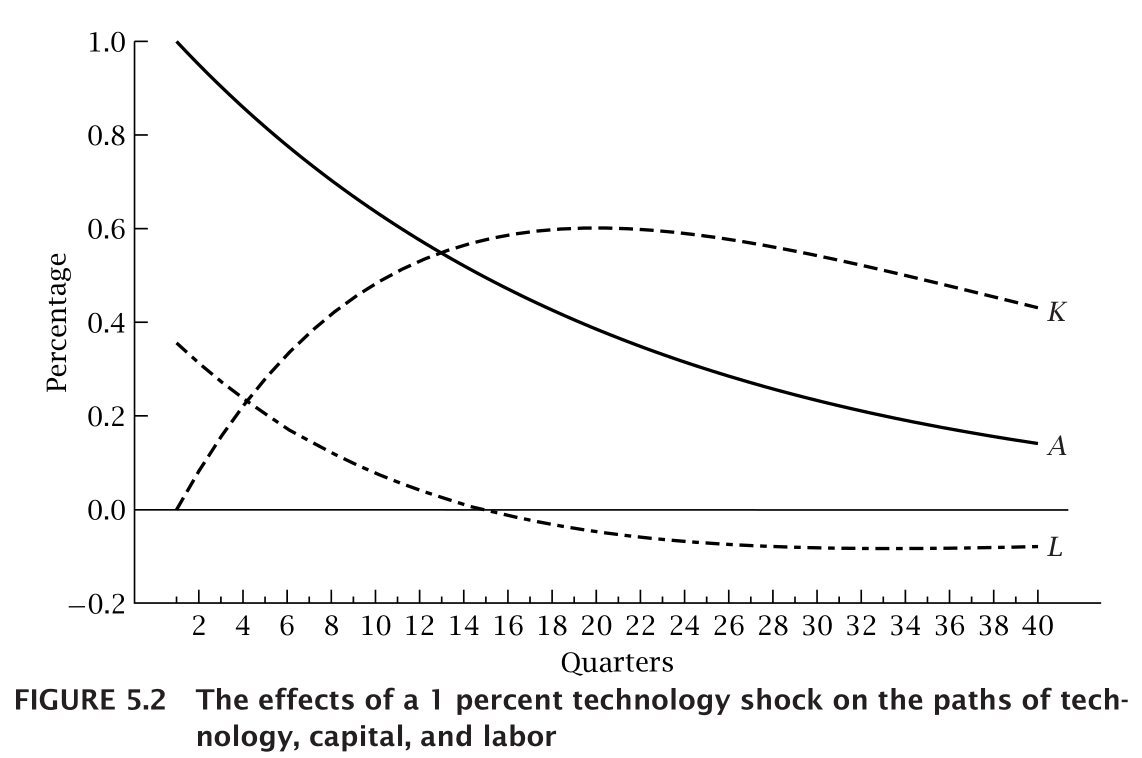
\includegraphics[scale = 0.35]{images/52}
\end{figure}
\begin{itemize}\footnotesize
\item Each period corresponds to a quarter
\item Baseline parameter values: \\ 
$\alpha=\frac{1}{3}, g=0.5 \%, n=0.25 \%, \delta=$ $2.5 \%, \rho_A=0.95, \rho_G=0.95$, and $\bar{G}, \rho$, and $b$ such that $(G / Y)^*=0.2, r^*=1.5 \%$, and $\ell^*=\frac{1}{3}$ \\ 
{\scriptsize{(See Problem 5.10 for the implications of these parameter values for the balanced growth path.)}}
\end{itemize}
\end{frame}

\begin{frame}
\frametitle{Technology shock: output and consumption}
\begin{figure}
\centering
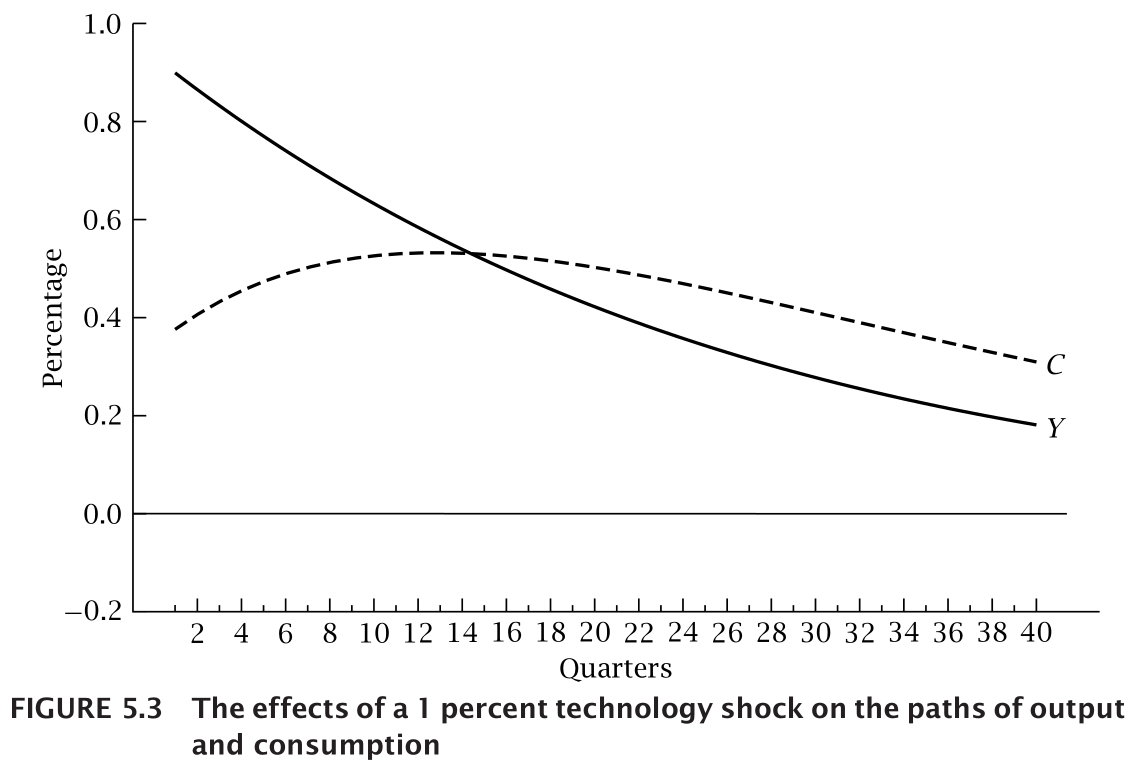
\includegraphics[scale = 0.35]{images/53}
\end{figure}
\end{frame}


\begin{frame}
\frametitle{Technology shock: wages and interest rate}
\begin{figure}
\centering
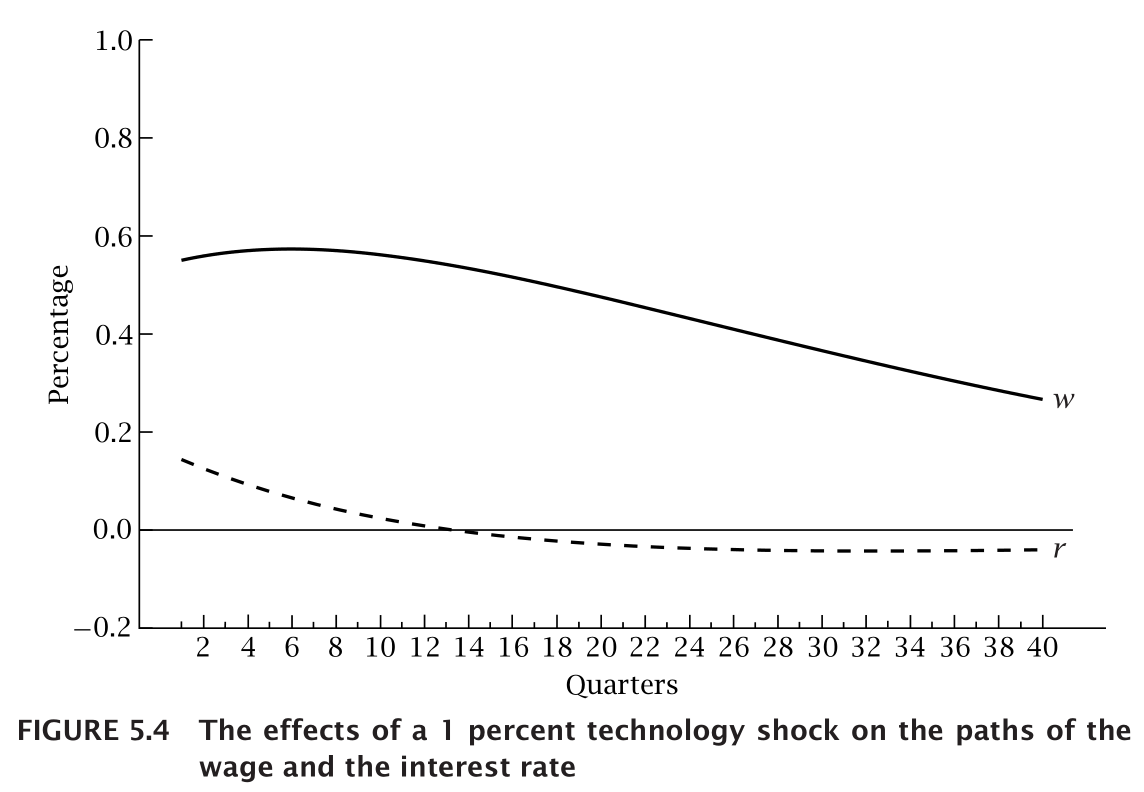
\includegraphics[scale = 0.35]{images/54}
\end{figure}
\end{frame}



\subsection{The effects of changes in government purchases}


\begin{frame}\frametitle{The effects of changes in government purchases}
\begin{itemize}
\item Intuitively, an increase in government purchases causes consumption to fall and labour supply to rise because of its negative wealth effects. 
\item And because the rise in government purchases is not permanent, agents also respond by decreasing their capital holdings.
\item See Figures 5.5-5.7 in Romer. Can you replicate this effect in the Tutorial? Bonus marks will be awarded.
\end{itemize}
\end{frame}



\section{Empirical application: calibrating an RBC model}

\begin{frame}\frametitle{Empirical application: calibrating a RBC model}

\vspace{0.5em}
\textbf{Key Steady-State Conditions (examples):}
\begin{align*}
    R &= \frac{1}{\beta} \quad \text{(Euler equation)} \\
    \frac{K}{Y} &= \frac{\rho}{R - (1 - \delta)} \quad \text{(MPK = R)} \\
    \frac{C}{Y} &= 1 - \delta \cdot \frac{K}{Y} \quad \text{(from resource constraint)}
\end{align*}
\vspace{0.5em}
\textbf{Interpretation:}
\begin{itemize}
    \item Capital-output and consumption-output ratios are pinned down by preferences and technology.
    \item Used to back out model parameters or to simplify coefficients in the linearised system.
    \item See Tutorial note for details.
\end{itemize}
\end{frame}

\begin{frame}\frametitle{From theory to simulation: what dynare computes}
\begin{itemize}
    \item \texttt{stoch\_simul(order=1)} solves the log-linearised model and computes:
    \begin{itemize}
        \item Theoretical moments: $\text{std dev}, \text{autocorr}, \text{corr with output}$
        \item Impulse Response Functions (IRFs)
    \end{itemize}
    \item These moments form the basis for empirical assessment in Romer (Ch. 5.10).
\end{itemize}
\vspace{0.5em}
\begin{block}{Tutorial}
    Students compare model-implied moments to empirical data from their chosen country.
\end{block}
\end{frame}



\begin{frame}
\frametitle{IRFs RBC Model (Matlab/Dynare)}
\begin{figure}
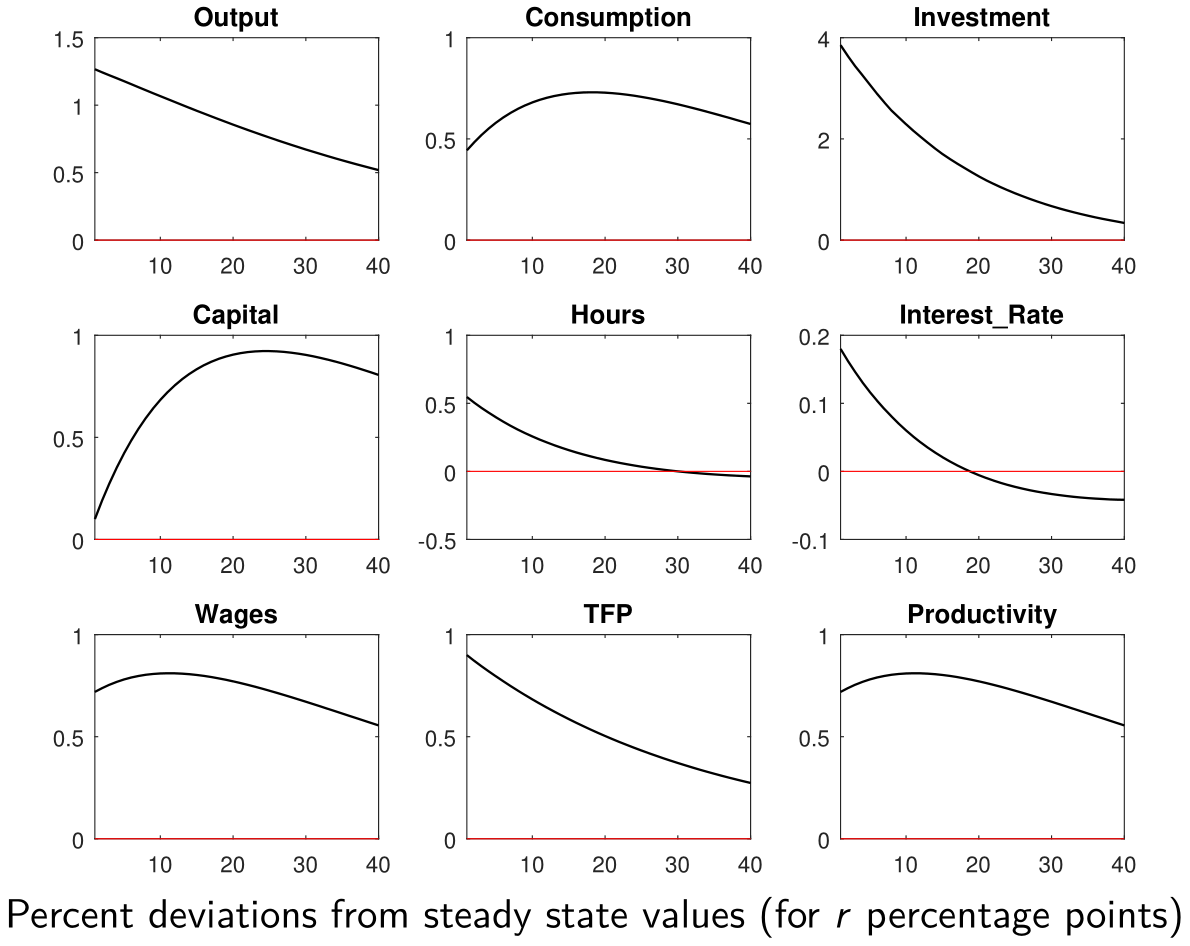
\includegraphics[scale = 0.37]{images/pol8}
\end{figure}
\end{frame}



\begin{frame}
\frametitle{Empirical application}
\begin{itemize}[<+->]
\item How do we decide if an RBC model matches the real world?
\item Normally we look at some of the following things:
\begin{enumerate}
\item Are relative amounts of cyclical variation in the variables correct?
\item Does the degree of persistence in each variable match its actual persistence?
\item Are the co-movements across variables realistic?
\end{enumerate}
\vspace{2mm}
\item The next slide shows how an RBC model compares to actual movements in the data, from \textbf{Plosser (1989)}.
\item His article is in the \emph{Journal of Economic Perspectives}, which is a great journal for less technical papers.
\end{itemize}
\end{frame}


\begin{frame}
\frametitle{Plosser's evidence}
\begin{figure}
\centering
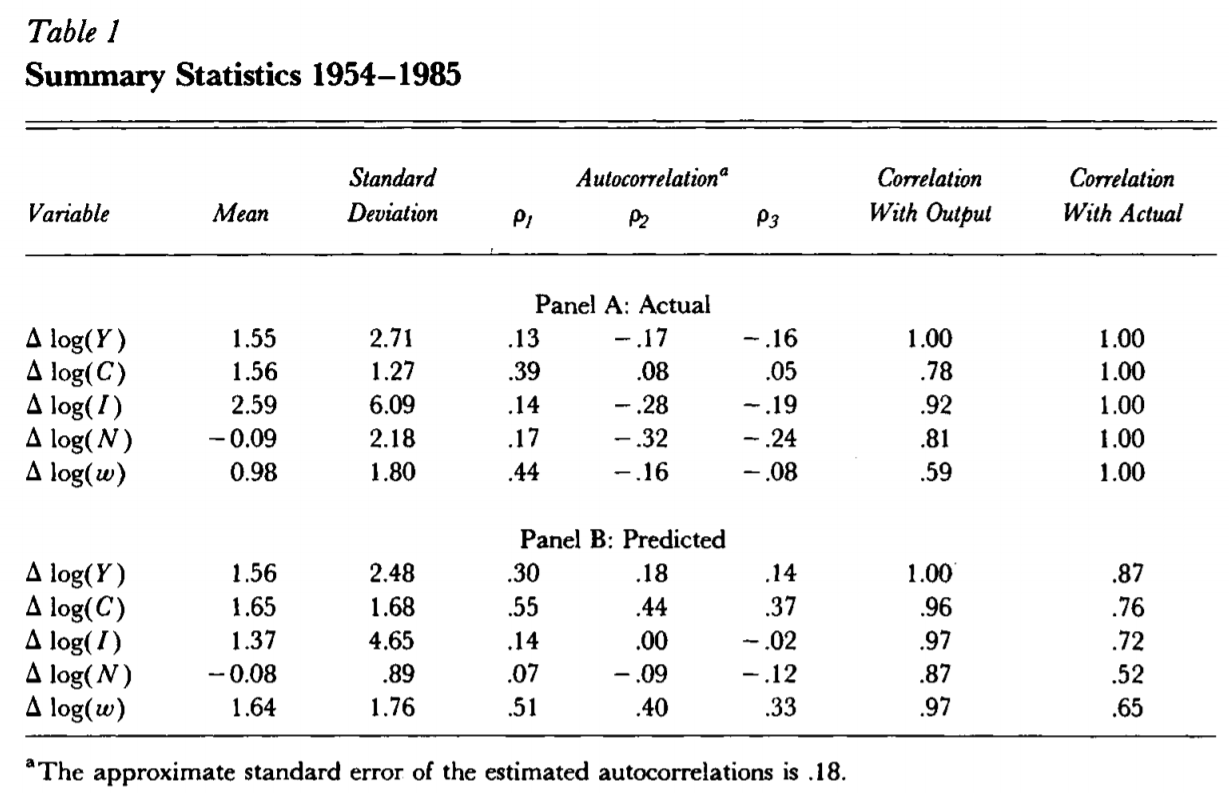
\includegraphics[scale = 0.35]{images/plosser}
\end{figure}
\end{frame}


\begin{frame}
\frametitle{Model vs data updated}
\begin{figure}
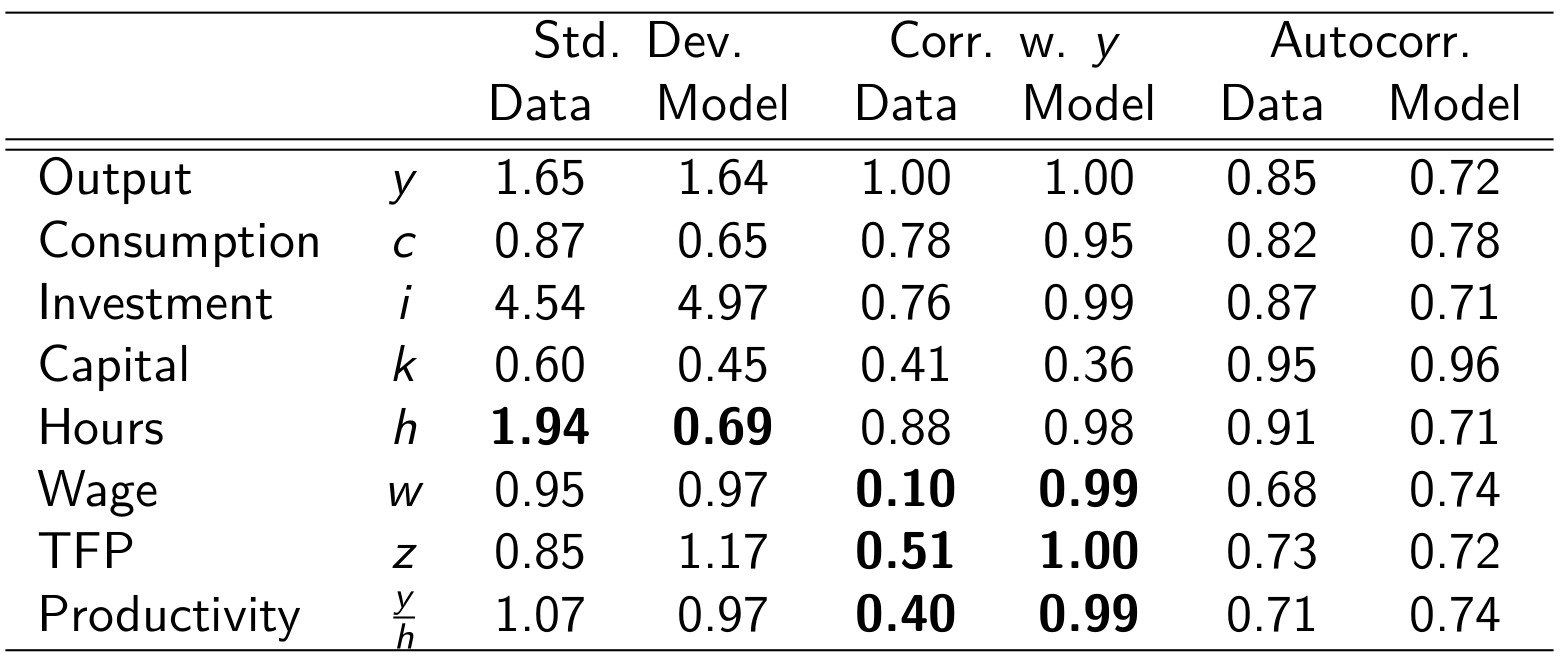
\includegraphics[scale = 0.33]{images/pol9}
\end{figure}
\end{frame}

\begin{frame}
\frametitle{Model vs data: Consumption}
\begin{figure}
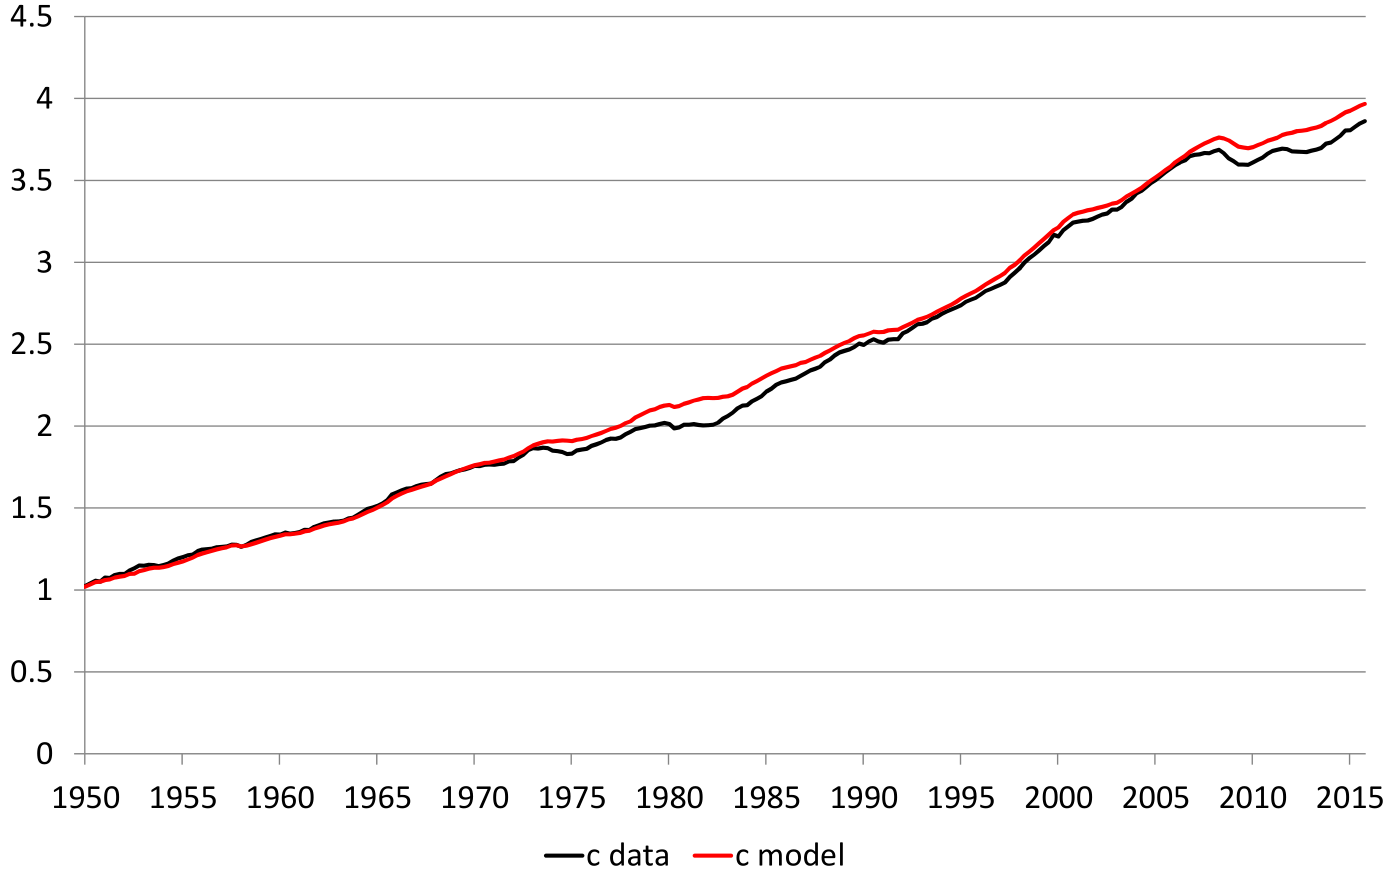
\includegraphics[scale = 0.33]{images/pol10}
\end{figure}
\end{frame}

\begin{frame}
\frametitle{Model vs data: Investment}
\begin{figure}
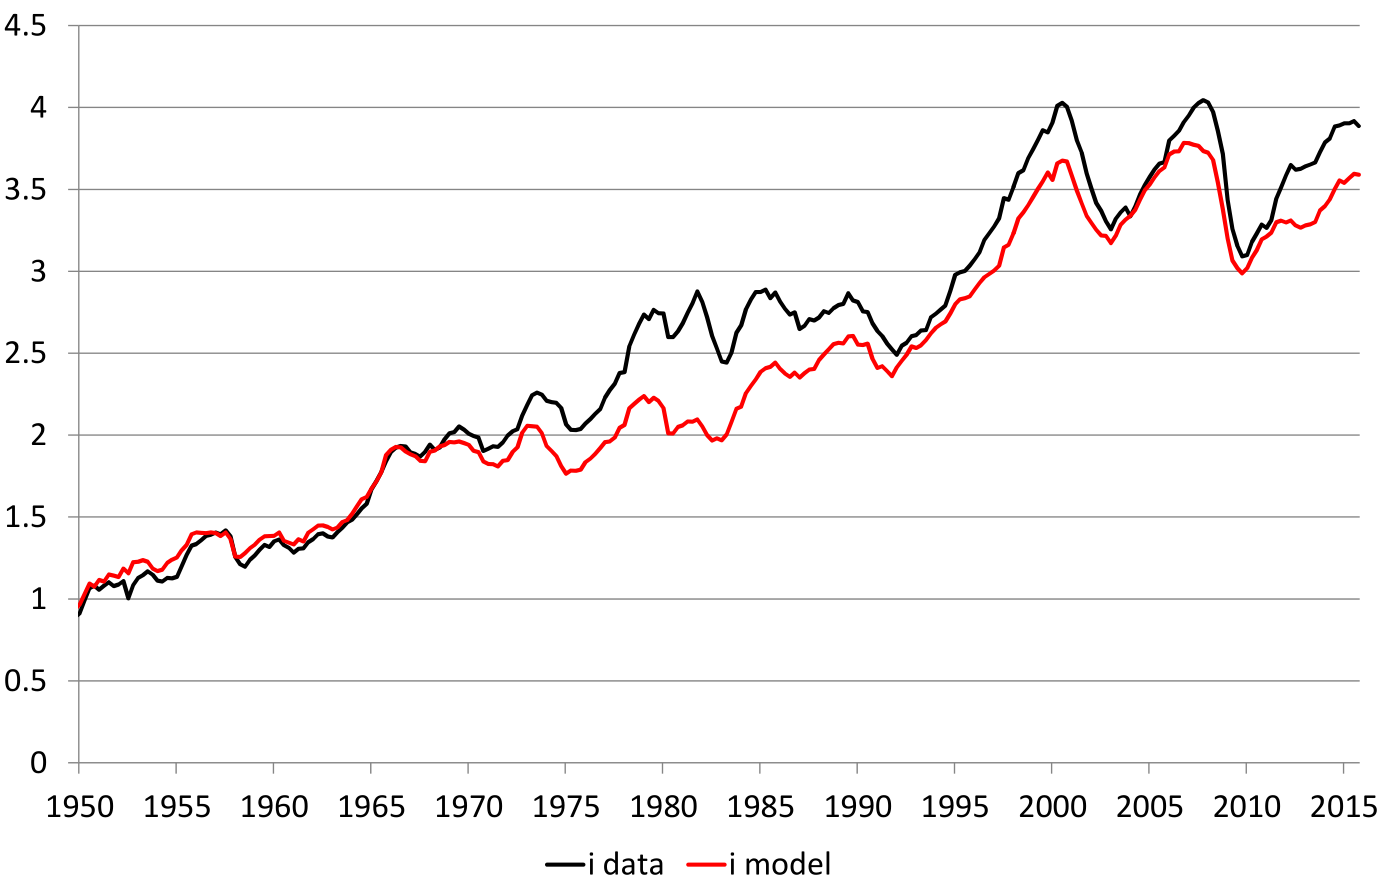
\includegraphics[scale = 0.33]{images/pol11}
\end{figure}
\end{frame}

\begin{frame}
\frametitle{Model vs data: Hours worked}
\begin{figure}
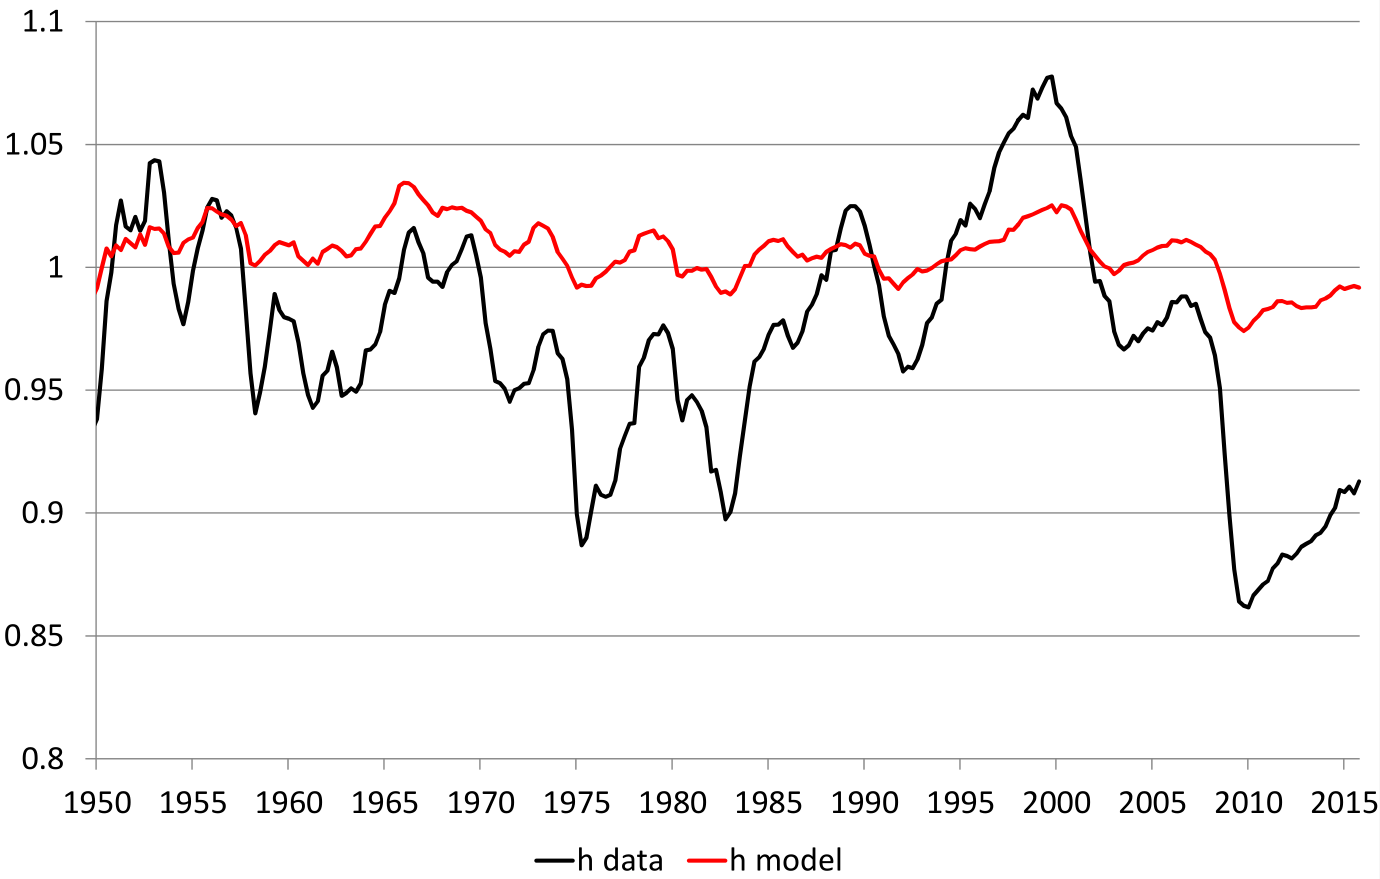
\includegraphics[scale = 0.33]{images/pol12}
\end{figure}
\end{frame}

\section{Assessing the baseline RBC model}


\begin{frame}
\frametitle{Assessing RBC models}
\begin{itemize}[<+->]
\item Looking at the table we can see some problems emerge:
\begin{itemize}
  \item Consumption and wages are too highly correlated with GDP
  \item Consumption, wages and output are too persistent
  \item Much too little variation in employment
\end{itemize}
\vspace{2mm}
\item The last point about variation in employment is worth discussing. Heavily debated in the literature.
\begin{itemize}
  \item RBC model explains employment fluctuations within a market clearing model (Walrasian)
  \item The change in employment must be on the labour supply curve
  \item If labour supply is \textbf{very elastic}, then we can have large changes in employment with small change in the wage
  \item However, \textcolor{blue}{micro evidence} shows that labour supply is quite inelastic! Complete opposite.
  \item Simple RBC model can't reconcile large $\Delta{L}$ with $\Delta{w} \ldots$
\end{itemize}
\vspace{2mm}
\item Basic RBC model does not seem to work for all cycles, but it might be useful for some $\rightarrow$ see, e.g., \textbf{Hamilton (2011)} and \textbf{Kehoe et al. (2018)}.
\end{itemize}
\end{frame}










\end{document} 